We evaluate our approaches on a wide variety of simulated scenarios, comparing the results against two benchmark solutions. For the first benchmark, we randomly generate detection assignments, including randomly assigning false alarms and missed detections for the case of detection ambiguity. This solution will be referred to as the \textit{random} solution. In the second benchmark, the detection assignments are known perfectly, meaning that all assignments are exactly correct including the classification of false alarms and identification of missed detections. This solution is referred to as the \textit{ideal} solution, however, it is only ideal in relation to the data association problem, but it provides a means for bounding the expected error in the trajectory estimation problem. Note that we do not compare our methods to any known MTT algorithms, such as the MHT or JPDAF, due to the complexity in tuning and the overhead of implementation of these algorithms. 

In the literature, there does not exist a clearly defined comprehensive set of standard test scenarios, as pointed out by \cite{MTT-Taxonomy}, which also notes that two types of scenarios of particular importance include crossing trajectories and parallel trajectories. Because we would like to test our methods across scenarios with a wide range of complexity, for both the data association and trajectory estimation problems, it is necessary to create scenarios using both methods. With this in mind, we choose to generate scenarios of both trajectory types using a simple methodology that will be outlined next in our discussion on experimental methods. 

We run two separate experiments, one with detection ambiguity and one without. Both experiments, including the scenario generation process, heuristic, and MIO, were implemented in the development software \textit{julia} 0.4.3 \cite{julia} using the optimization package \textit{JuMP} \cite{JuMP}. The optimization software Gurobi 6.5.0 \cite{gurobi} was used to solve the MIOs, and the optimization processes was restricted to the use of a single core. Each simulation was run on a single compute node of the unclassified TX-Green cluster located at Lincoln Laboratories. The cluster utilizes DL165 G7 compute nodes, consisting of 2.2 GHz compute cores, with 8 GB of RAM each, for a total peak performance of 77.1 TFLOPS \cite{LLGrid}. 

We begin by outlining our experimental methods for scenarios without detection ambiguity and discuss the results of our approaches on these scenarios. 

\mysubsection{Scenarios without Detection Ambiguity}
In order to evaluate scalability of our algorithms we test our methods across a range of scenarios with varying numbers of targets and scans. In particular we consider $ P \in \{4,6,8,10\}$ targets and $T \in \{4,6,8,10\}$ scans. The scans are collected at a rate of 1 Hz. The cartesian product of $P$ and $T$ creates 16 unique scenario sizes. We generate 10 unique crossing scenarios and 10 unique parallel scenarios of each size. 

To generate trajectories, we first establish a state space as the segment $[-\tau,\tau]$. For our experiments, we elected for $\tau = 20$. Two points within this state space are selected to define a trajectory, where the first is referred to as the trajectory's \textit{initial position} and the second as the trajectory's \textit{final position}. To generate crossing trajectories, the initial and final positions are randomly selected from within the full range of the state space. To generate parallel trajectories, the state space is divided into $P$ equal non overlapping segments, such that within the $i$th segment we randomly select the initial and final positions for target $i$. This ensures the generation of trajectories that do not cross or overlap, but will remain within close proximity of each other. 

For each scenario, we randomly generate 10 realizations of data by first perturbing each true position measurement by an error $\epsilon \thicksim \mathcal{N}(0,\sigma)$ with $\sigma \in \{0.1,0.5,1.0,2.0,3.5,5.0\}$, where $\sigma$ represents the noise parameter. Adding the detection error to the true position results in a detection:
\begin{align*}
	x_{it} = \alpha^{\text{true}}_{i} + \beta^{\text{true}}_{i}t+\epsilon.
\end{align*}

Scans $\mathcal{X}_{t}$ are simulated by randomizing the order of $x_{it}$ for each \textit{t}. Each unique $\boldsymbol{\mathcal{X}}$ generated is referred to as a \textit{simulation}. For each such simulation, we run the heuristic with a range of number of starting points $N \in \{100\ \ 1,000\ \ 10,000\}$, and use each of these solutions as a warm start for the MIO. The optimization process is set to terminate after 3T seconds, with solutions collected at intervals of $\{1,T,2T,3T\}$ seconds.

At the conclusion of the experiment, we calculated the difficulty of each scenario, the accuracy of each solution, and the trajectory estimation error $\delta$. When measuring the difficulty of scenarios in terms of $\rho$, we propose the use of $h(\sigma)=2\sigma$, since it is difficult to distinguish detections which lie between target trajectories that are closer.

\mysubsubsection{Scenario Generation}
We begin with a discussion on the relationship between $\rho$ and $\sigma$ and show how this relationship benefits both scenario generation and complexity measuring by allowing each to occur in their own natural domain. Figure~\ref{fig:Sigma_vs_Rho} shows the relationship between $\sigma$ and $\rho$ for the 20 scenarios simulated in our experiments. The plot is broken down by scenario type between crossing and parallel trajectories. 
\begin{figure}[ht]
  \centering
  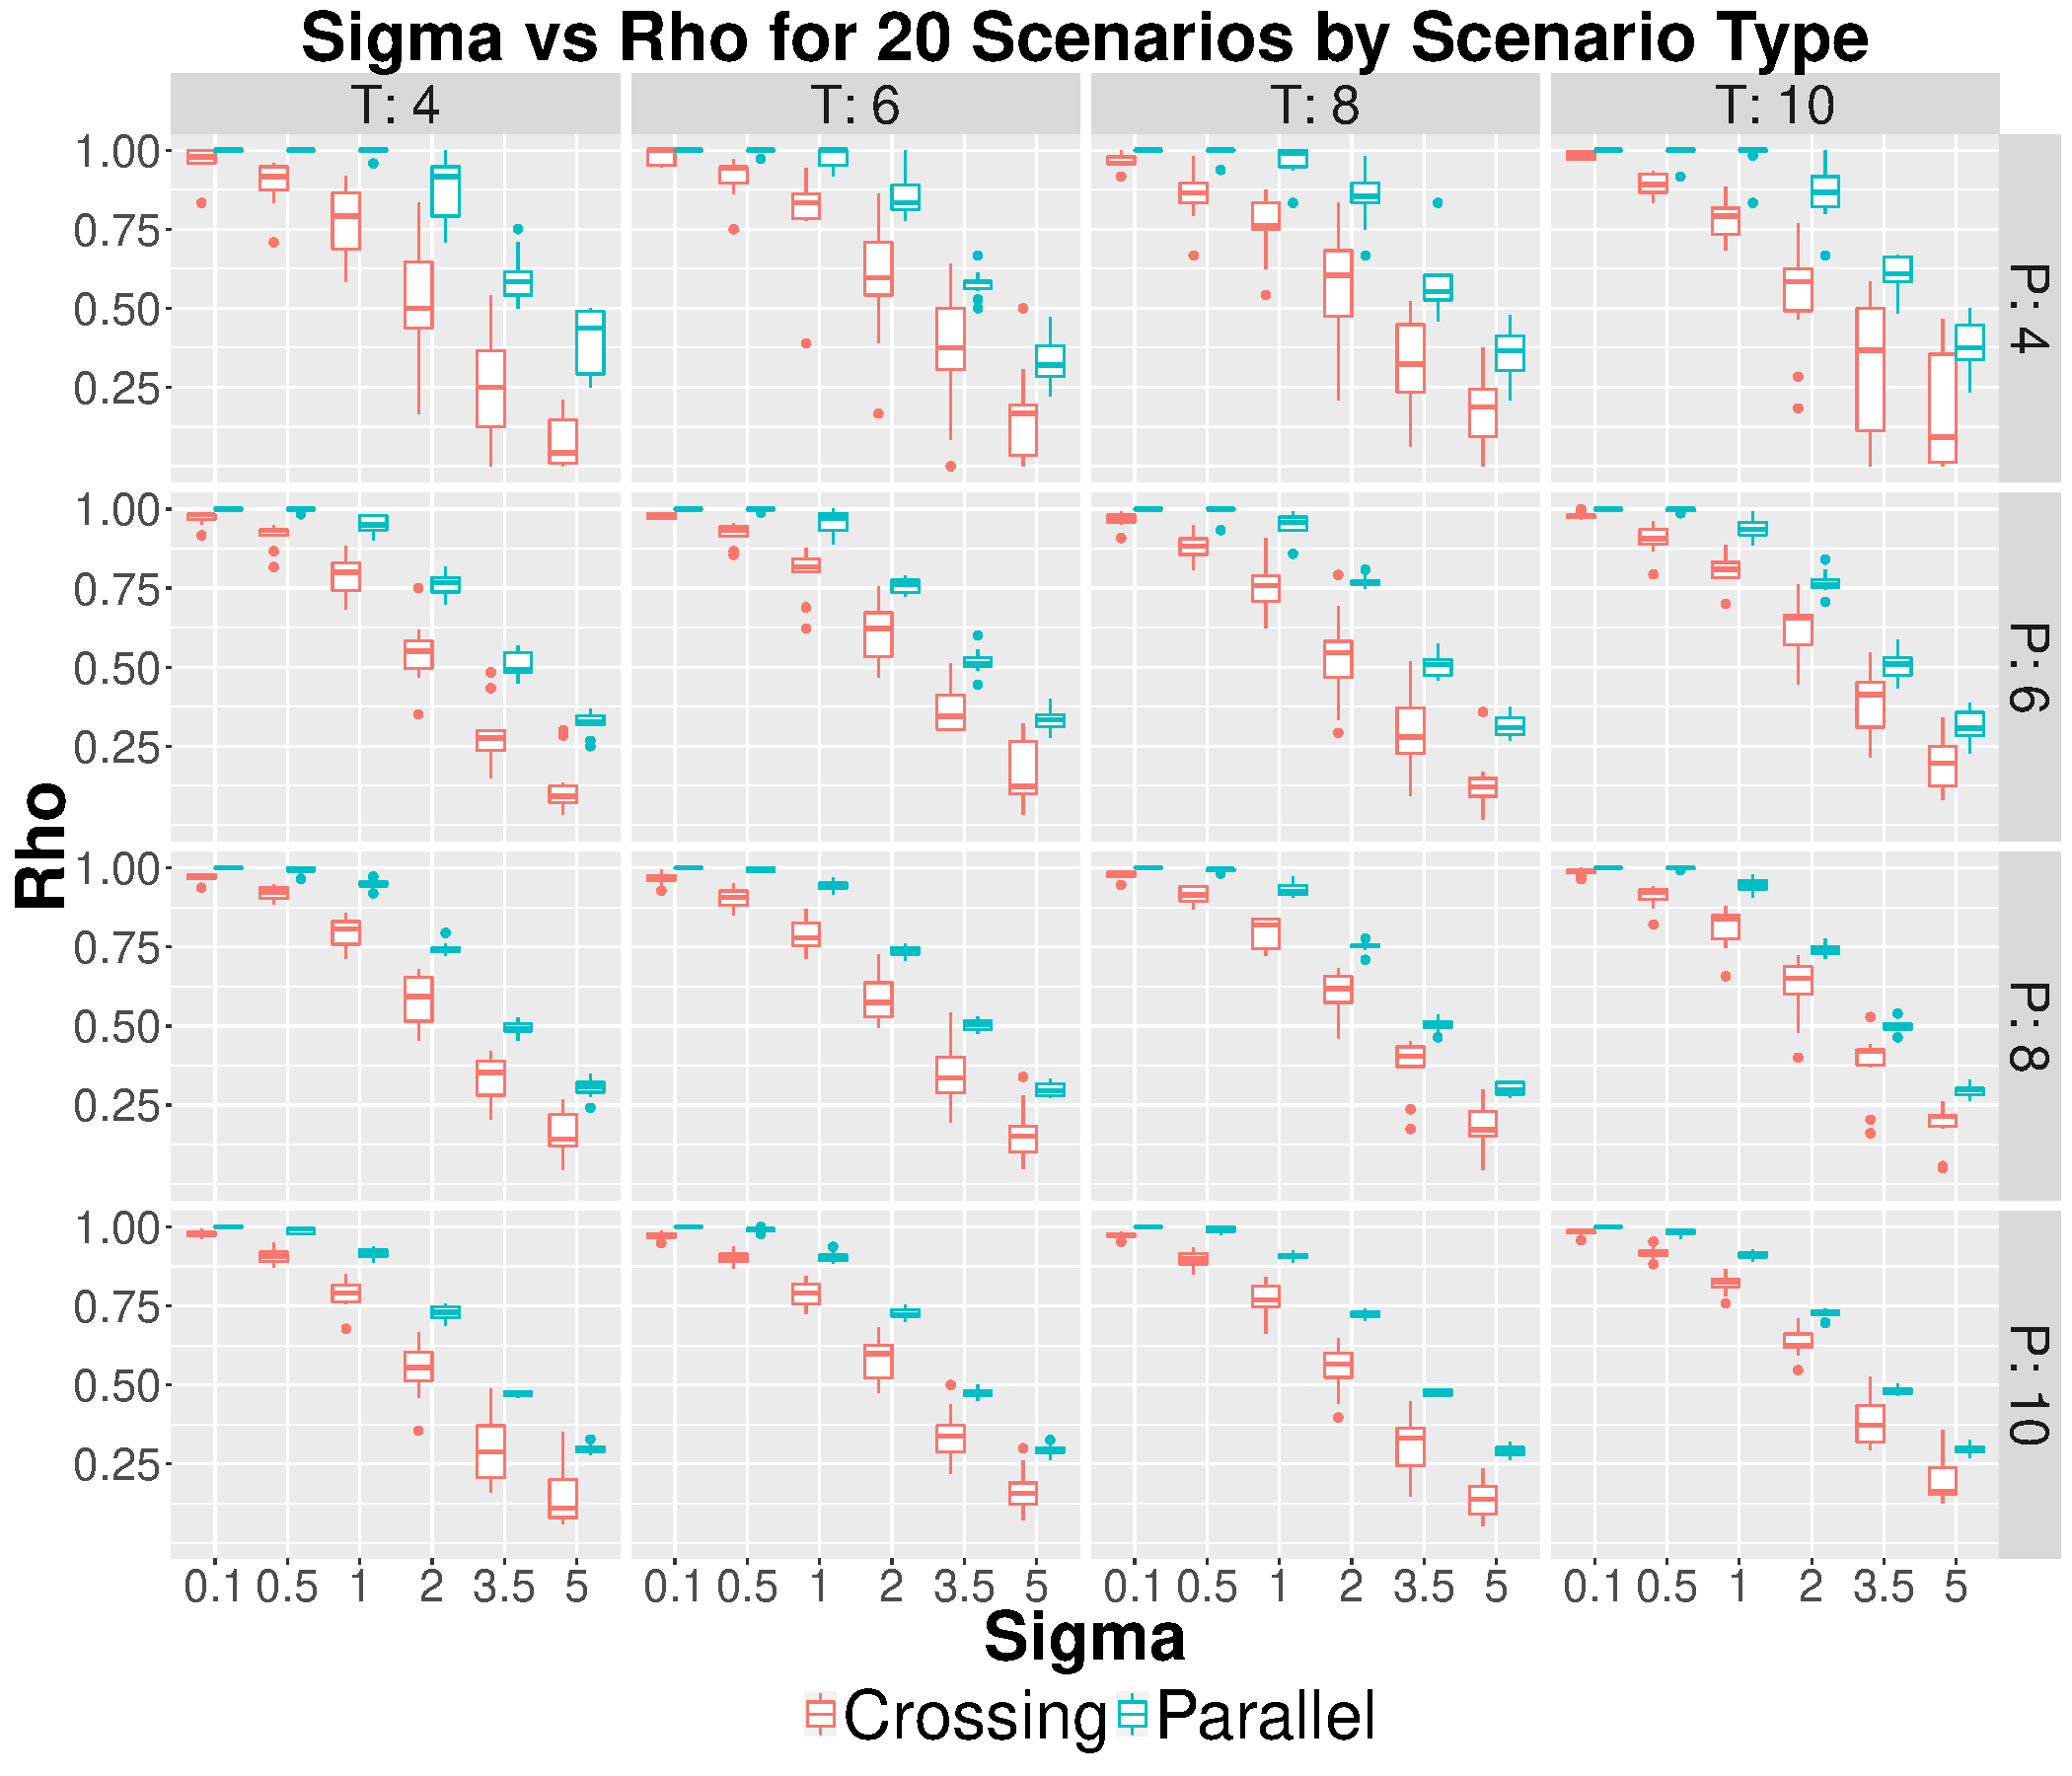
\includegraphics[width=\columnwidth]{../Figures//Sigma_vs_Rho}
    \caption{Relationship between $\sigma$ and $\rho$ summarized by scenario type for all 20 generated scenarios in this experiment.}
    \label{fig:Sigma_vs_Rho}
\end{figure}

Remember that higher values of $\rho$ indicate a lower proportion of detections within very close proximity to one another. We note that the parallel method of scenario generation clearly generates easier scenarios, as measured by $\rho$. This suggests that it may be more difficult to discern correct associations for crossing scenarios than for parallel scenarios. In addition, we can conclude from Figure~\ref{fig:Sigma_vs_Rho} that $\sigma$ and $\rho$ are highly correlated, and the higher $\sigma$ is the lower $\rho$ becomes, which in to be expected from the definition of $\rho$. 

We also note that the range of $\rho$ values corresponding to a single value of $\sigma$ decreases as the number of targets increases. In other words, as the number of targets increases, it becomes more difficult to generate a wider variety of $\rho$ values from a given $\sigma$. For example, for the crossing scenarios with $T=10$ and $\sigma=5$, in the case of four targets the range of $\rho$ is approximately while $[0,0.5]$, while  in the case of ten targets it is limited to $[0.125,0.375]$. Most likely, this is a result of using a fixed state space, as the number of target increases the flexibility of positioning the track decreases.

 Although the variety of difficulty measures decreases as the number of targets increases, the measure $\rho$ still provides a meaningful measure of difficulty for the data association problem. 

\mysubsubsection{The Basic Heuristic Scalability}
We transition to evaluate the scalability of the heuristic run times. Table~\ref{tab:Basic_heuristic_times} summarizes the minimum, mean, and maximum run times of the heuristic for a single starting point, arranged by the number of targets ($P$) and number of scans ($T$). Times are shown in milliseconds. 

\begin{table}[ht]
\centering
\begin{tabular}{cc|ccc}
  \hline
   & & \multicolumn{3}{c}{Basic Heuristic Run Times } \\
   & & \multicolumn{3}{c}{(in milliseconds)}\\
   P & T & $\;\;$Min$\;\;$ & Mean & Max \\ 
  \hline
  \hline
   4 & 4 & 0.07 & 0.10 & 0.18 \\ 
   4 & 6 & 0.18 & 0.24 & 0.38 \\ 
   4 & 8 & 0.34 & 0.45 & 0.62 \\ 
   4 & 10 & 0.58 & 0.76 & 1.02 \\ 
   6 & 4 & 0.11 & 0.15 & 0.25 \\ 
   6 & 6 & 0.31 & 0.39 & 0.58 \\ 
   6 & 8 & 0.64 & 0.81 & 1.05 \\ 
   6 & 10 & 1.24 & 1.56 & 2.02 \\ 
   8 & 4 & 0.14 & 0.19 & 0.30 \\ 
   8 & 6 & 0.46 & 0.57 & 0.86 \\ 
   8 & 8 & 0.95 & 1.24 & 1.58 \\ 
   8 & 10 & 2.07 & 2.53 & 3.37 \\ 
   10 & 4 & 0.19 & 0.25 & 0.41 \\ 
   10 & 6 & 0.63 & 0.80 & 1.03 \\ 
   10 & 8 & 1.44 & 1.84 & 2.44 \\ 
   10 & 10 & 2.96 & 3.73 & 4.56 \\ 
   \hline
\end{tabular}
\caption{Heuristic run times (in milliseconds) for a single starting point.}
\label{tab:Basic_heuristic_times}
\end{table}

Close examination shows that the heuristic scales more efficiently with increases in the number of targets than increases in the number of scans. For example, increasing from four to six scans for four targets increases the computational cost by $140\%$, while increasing from four to six targets for four scans increases the computational cost by $50\%$. The same trend holds true across all targets and scans. Although the heuristic scales more efficiently in $P$ than $T$, the heuristic does not exceed 5 milliseconds in all cases per starting point.

The true scalability of the heuristic is fully realized when we consider the power of parallelization. By running the heuristic on several processors, we can reduce the number of starting points run on each processor, and in turn reduce the total running time. As a result, given enough processors, the heuristic can run several thousand starting points and still find solutions in a fraction of a second. To illustrate this, say that we intend to run 50,000 heuristic starting points for a scenario with six targets and six scans. The average run time for a single starting point of this size is about 0.4 milliseconds. Running all of these starting points in sequence would require approximately 20 seconds of run time, however, those same starting points parallelized onto 100 processors would only require a run time of 0.2 seconds. Thus, the run time of the heuristic can be reduced to meet the efficiency needs of the system, subject only to the limitation of available processors. 

In order to determine the appropriate number of starting points for the heuristic, we examine the MIO objective value of heuristic solutions for various number of starting points, recall that regardless of the number of starting points we will always choose the solution with the best objective function value. For ease of notation, let $f_{H}$ be the MIO objective score of the heuristic solution and $f_{I}$ be the MIO objective score of the ideal solution, which as a reminder is the solution in which the data association problem is exactly correct. We then compute the ratio of $f_{H}/f_{I}$, providing us a normalized measure for comparing the objective score across several scenarios. Figure~\ref{fig:Basic_Heuristic_Objective} plots $f_{H}/f_{I}$ (log scale)  against $\sigma$.
\begin{figure}[ht]
  \centering
  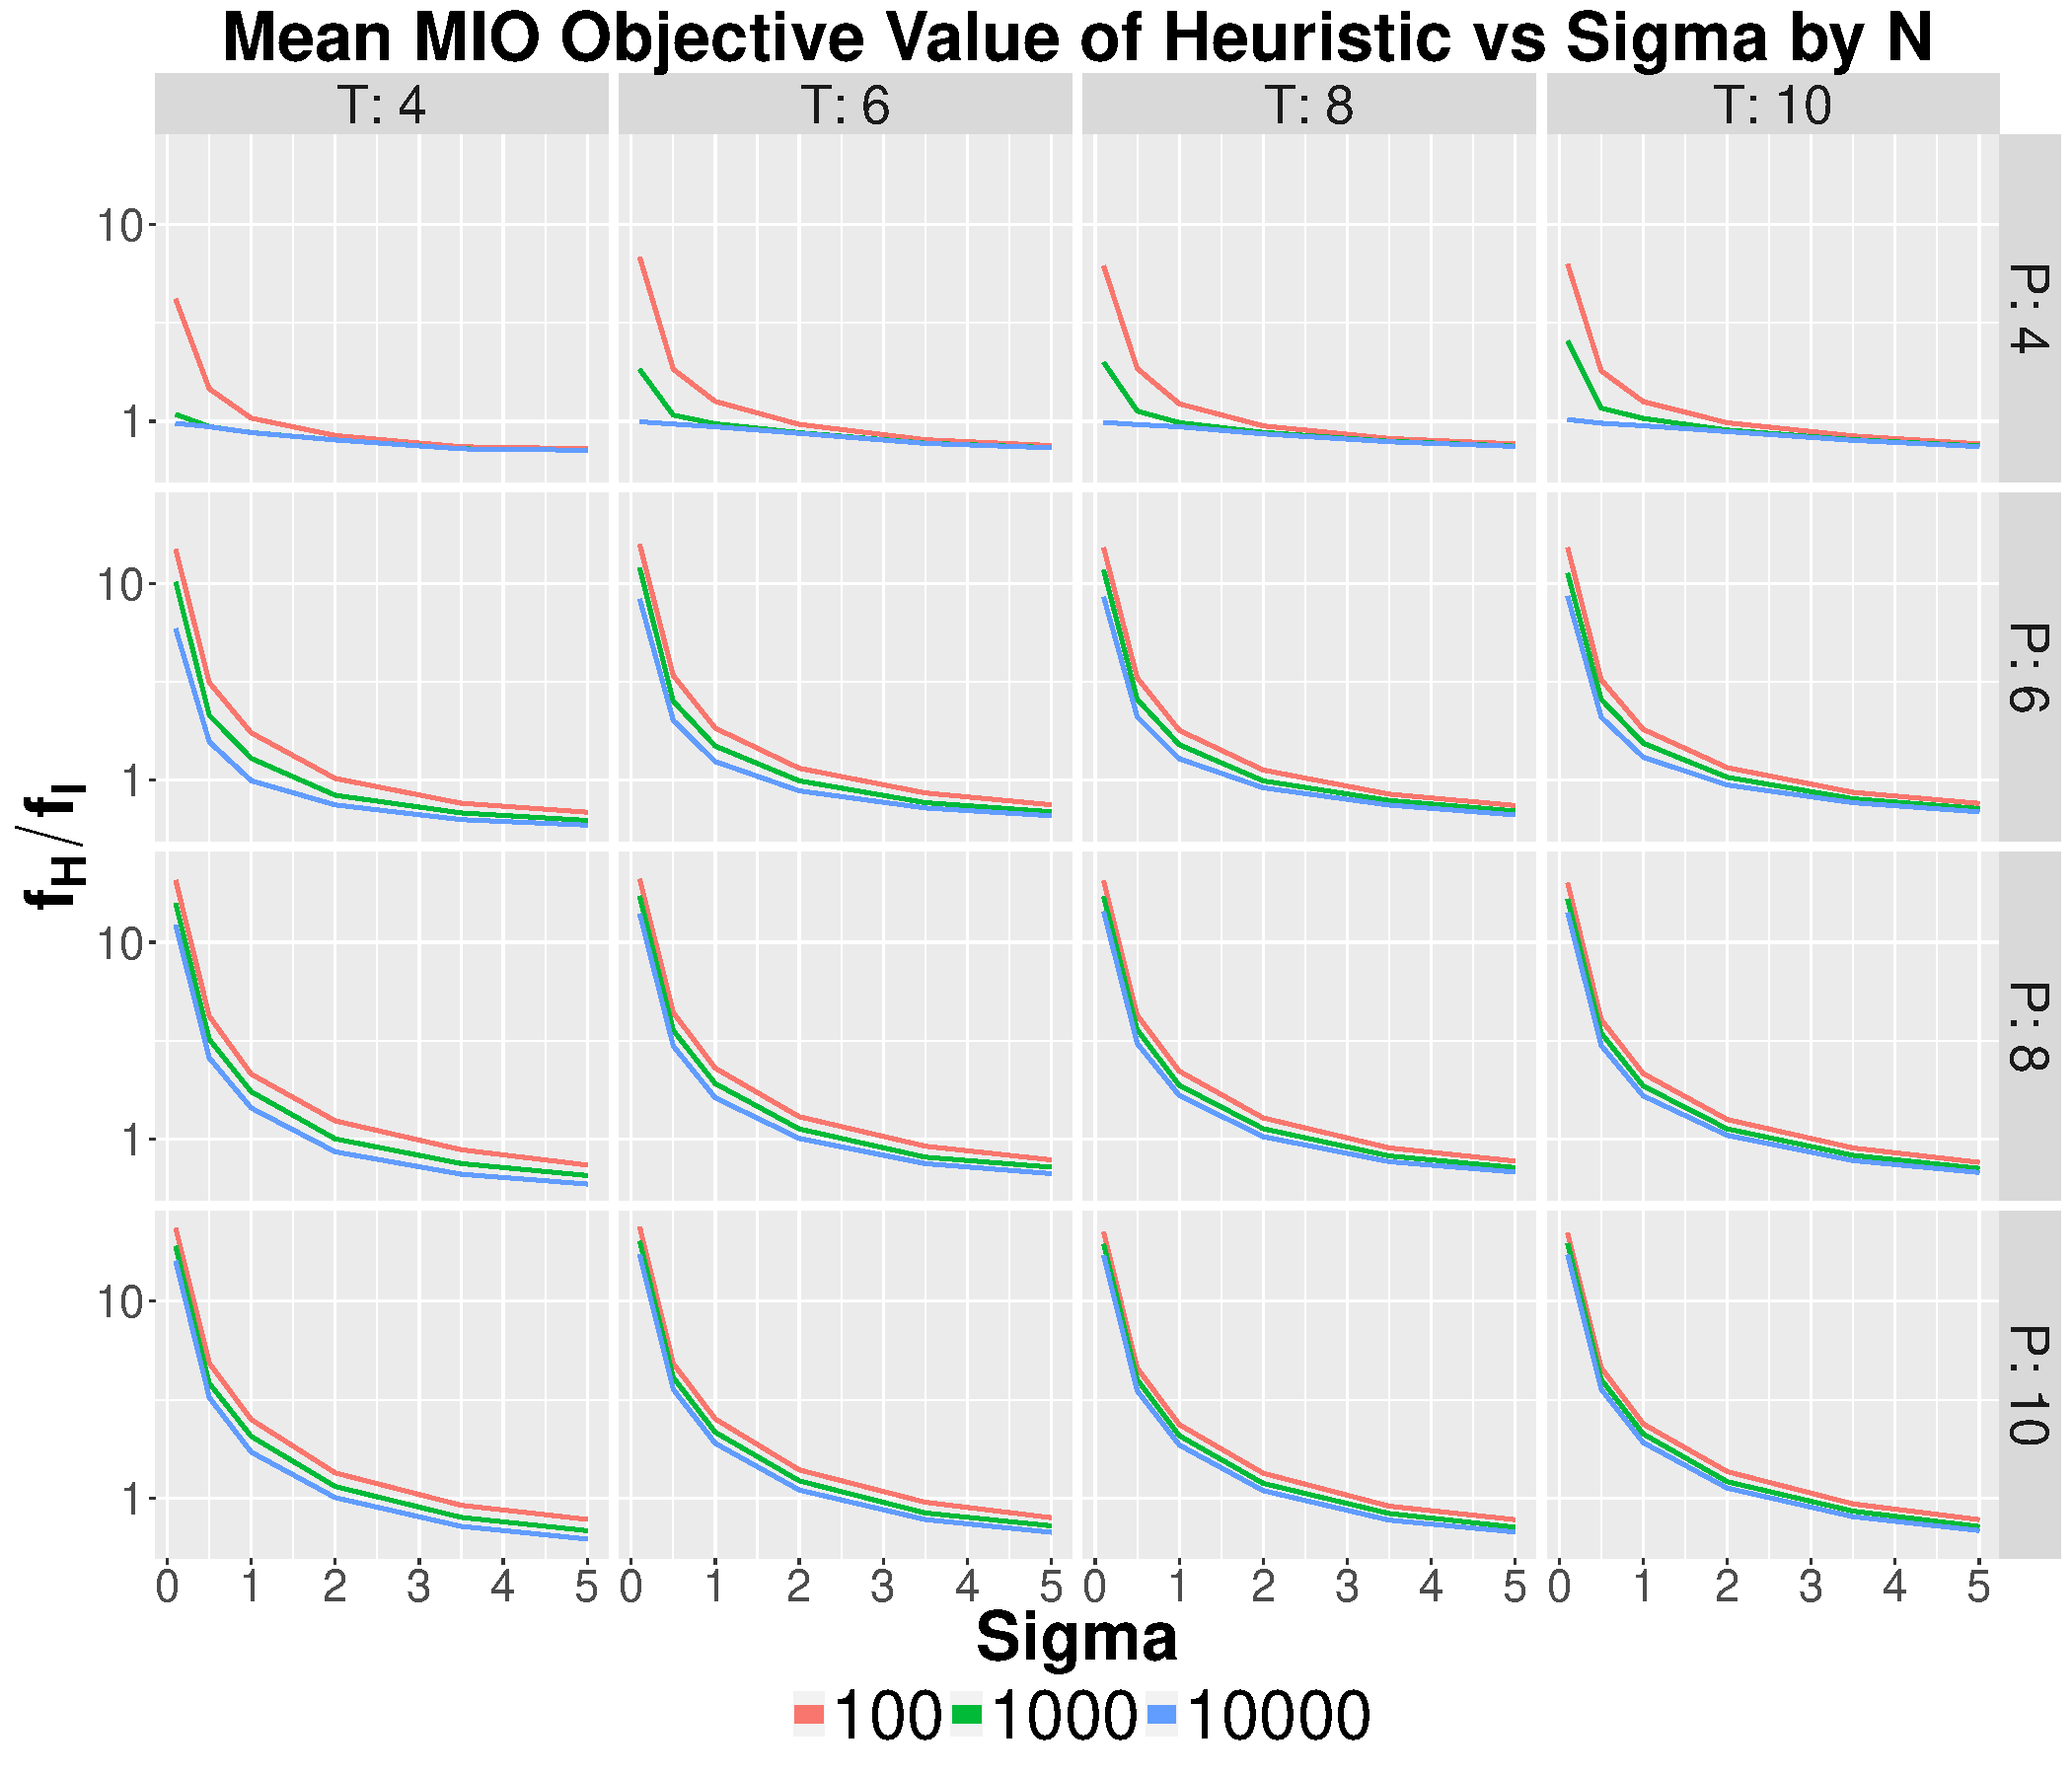
\includegraphics[width=\columnwidth]{../Figures/Basic_Heuristic_Objective}
  \caption{Quality of heuristic solution as compared to the ideal solution's MIO objective value summarized by number of starting points.}
  \label{fig:Basic_Heuristic_Objective}
\end{figure}

In all cases, increasing the number of starting points improves the heuristic solution as compared to the ideal solution. For scenarios of four targets, the improvement is greatest, on the order of about five times improvement from 100 to 10,000 starting points. However, for scenarios with more targets, there is only slight improvement in objective value with increases in the number of starting points. This suggests that in order to improve MIO objective value, the number of necessary starting points increases with $P$, likely due to the exponential increase in combinatorial solutions as the number of targets increases. In any event, we have seen that there is not a significant difference in heuristic performance for the range of $N$ values that we explored. Therefore, for simplification as we move forward in our analysis, we will restrict our discussions of the heuristic to $N=1,000$. 

It is also interesting to note that in some instances the ratio $f_{H}/f_{I}$ falls below the value 1, indicating that the heuristic outperforms the ideal solution, as measured by the objective function. This occurs for higher values of $\sigma$, for example, when the value of $\sigma$ is larger than $2$ regardless of the value of $P$ and $T$. To explain this phenomenon, we must recall that the ideal solution is simply ideal in the sphere of data association, while the MIO objective function serves to provide a measure of solution quality in regards to both data association and trajectory estimation. This seems to suggest that it may be necessary to tradeoff correct data associations in order to improve the trajectory estimation in cases where there is more detection noise. 

With these points in mind we continue our analysis to evaluate solution quality for both the data association problem and trajectory estimation for both the heuristic and MIO solutions.

\mysubsubsection{Data Association}
We shift our focus to analyze the performance of both the basic heuristic and the basic MIO model in regards to the data association problem. Figure~\ref{fig:Basic_Accuracy_Summary} plots the mean accuracy of both solutions against $\rho$, our measure of difficulty for data association. The heuristic shown on the plot was initialized with 1,000 starting points and the MIO model was provided this solution as a warm start. Note that the results for the MIO model do not include the solution at $3T$ seconds, since it exhibited little to no improvement over the MIO solution at $2T$ seconds. The ideal solution, which always achieves an accuracy of 1.0, has also been excluded for the sake of clarity.
\begin{figure}[ht]
  \centering  
  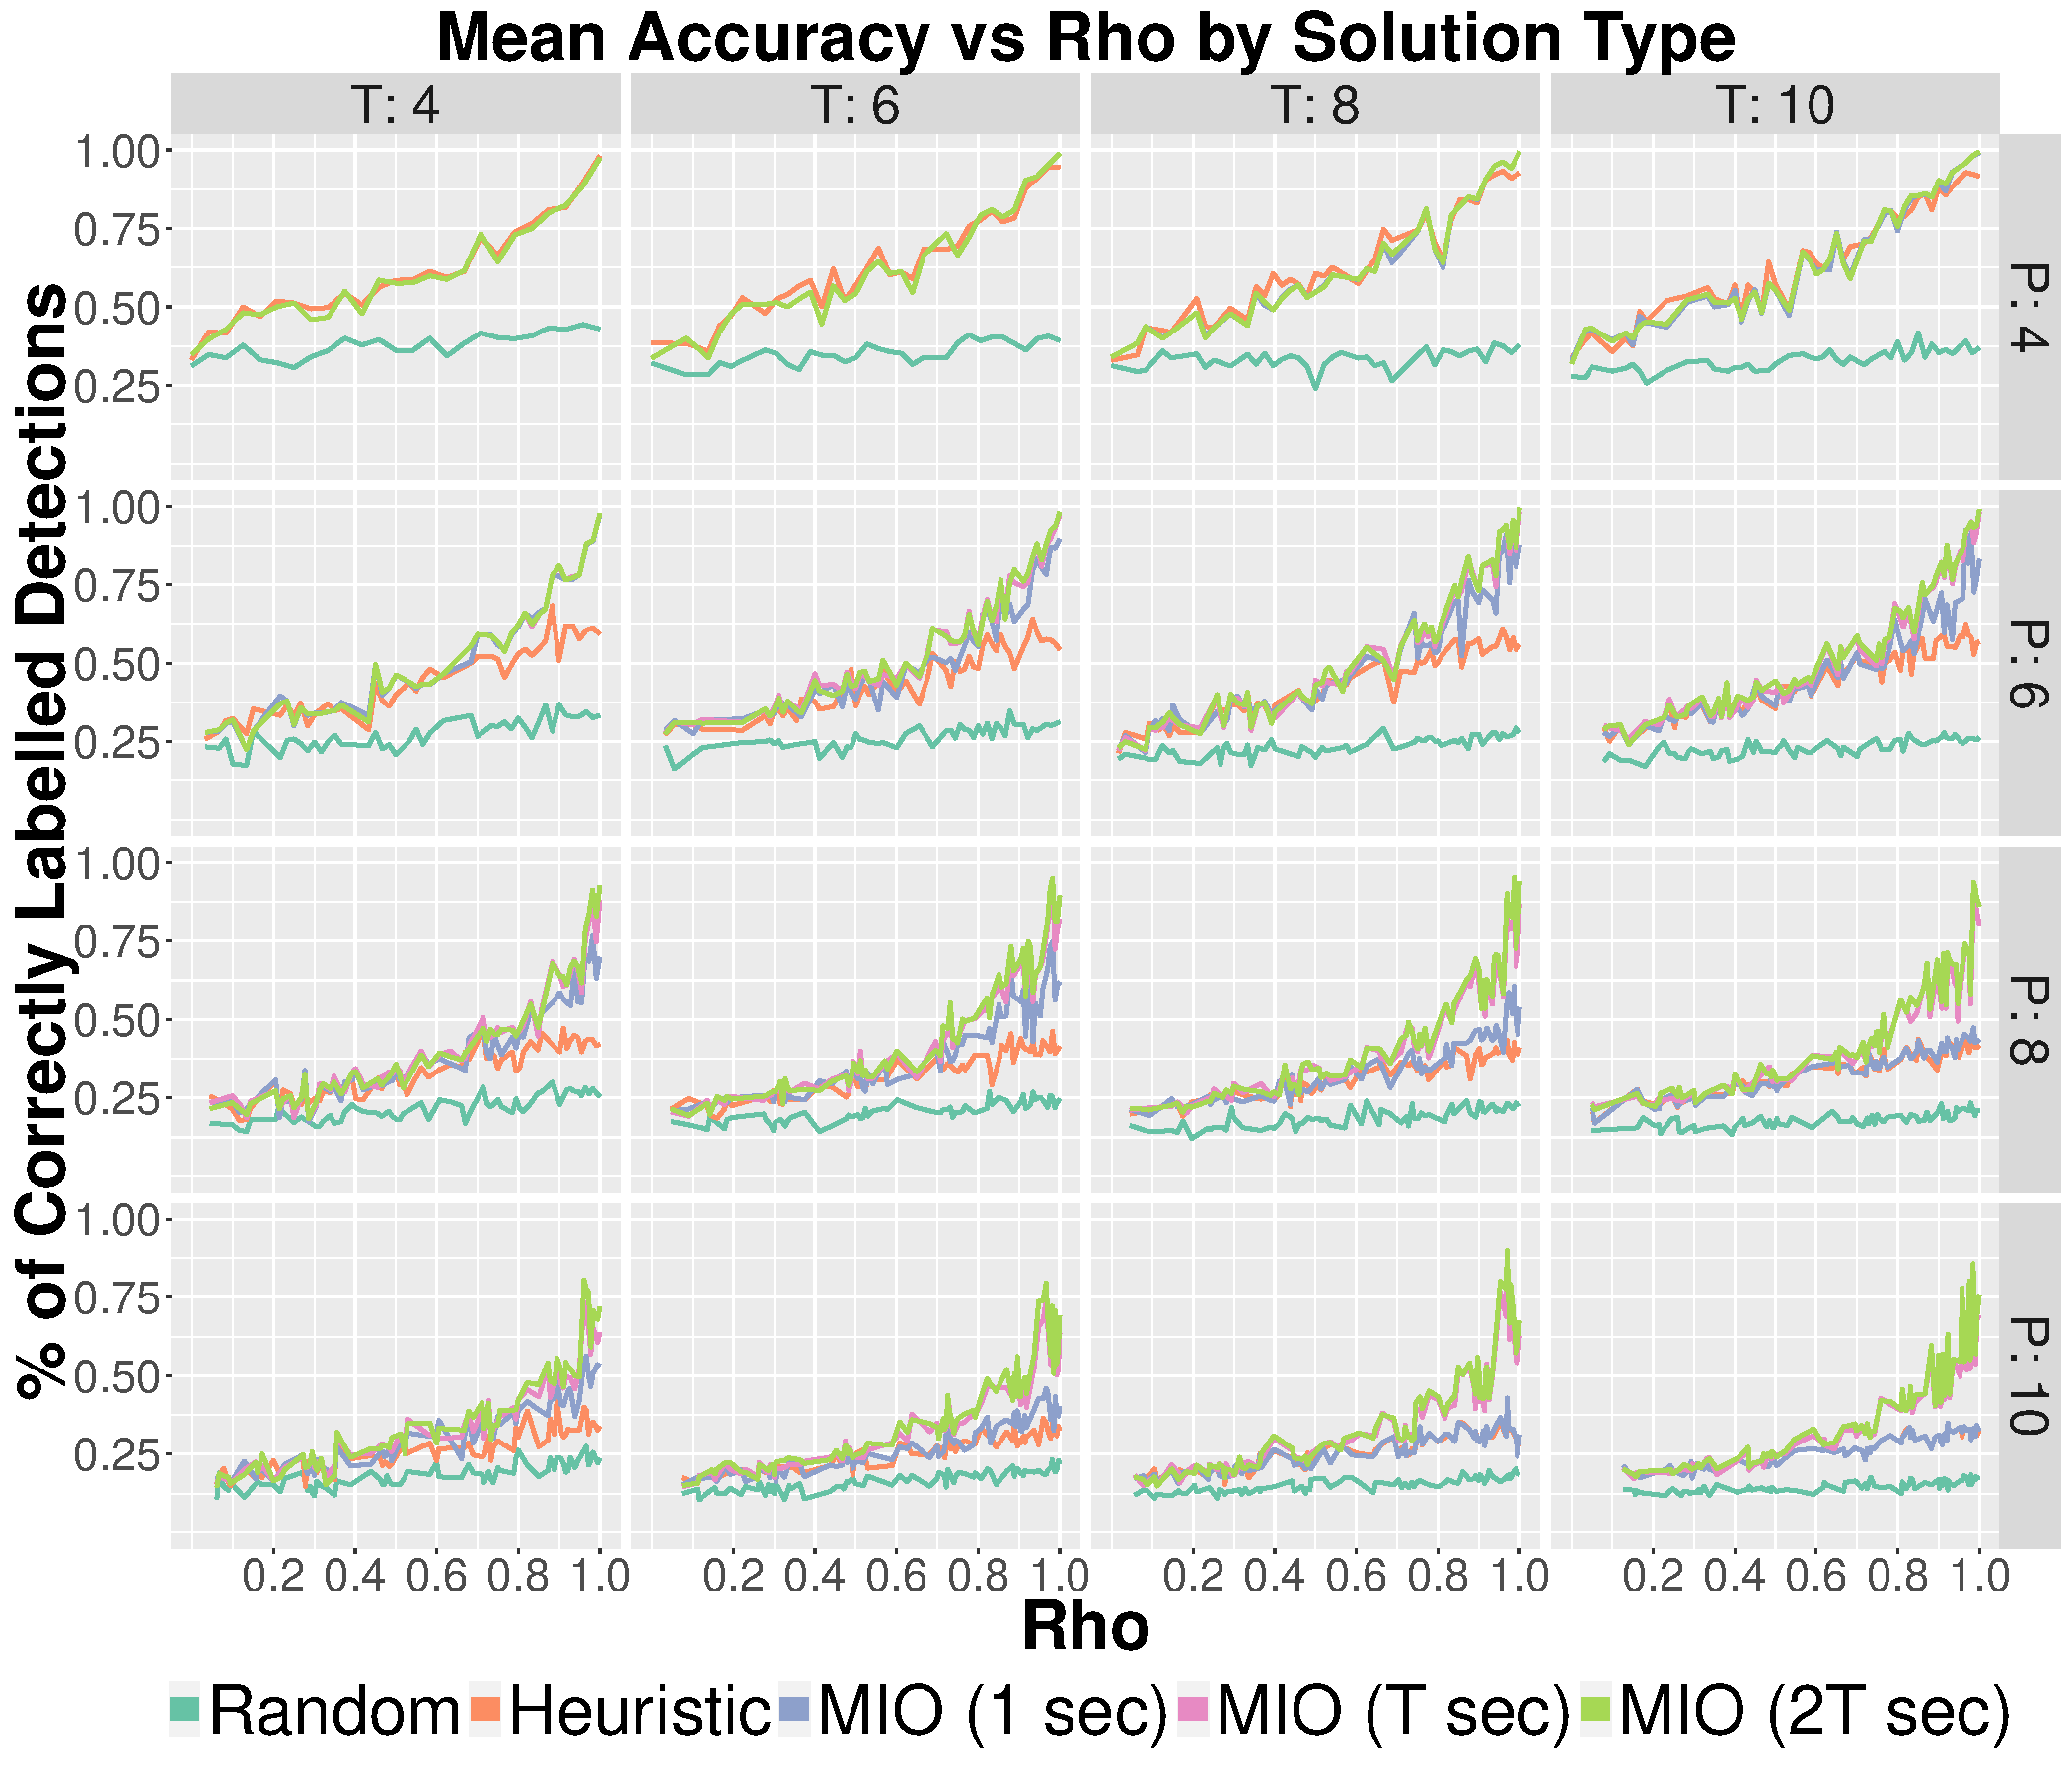
\includegraphics[width=\columnwidth]{../Figures/Basic_Accuracy_Summary}
  \caption{Accuracy of MIO compared against the heuristic and a randomized solution.}
  \label{fig:Basic_Accuracy_Summary}
\end{figure}

Figure~\ref{fig:Basic_Accuracy_Summary} shows that the quality of the associations found by both the heuristic and the MIO are indeed highly correlated with the scenario complexity parameter $\rho$, and the number of correct association in both increase as $\rho$ reaches $1$. Where for 4 and 6 targets the association is extremely close or exactly the ideal association, when $\rho$ is equal to $1$. In contrast the random association is unaffected by the value of $\rho$ and it accuracy is always lower than the heuristic accuracy. 

In general, it seems that running the MIO for $T$ or less seconds is optimal, since longer running times do not improve the accuracy attained. Specifically, for scenarios of four targets, the best accuracy is reached after $1$ second, while for scenarios of eight and ten targets, the best accuracy is reached after $T$ seconds. 

In scenarios of all sizes, the heuristic improves over the random solution, suggesting that the heuristic finds good quality solutions. In fact, for scenarios of four targets, the heuristic performs equally as well as the MIO model across all numbers of scans. While for scenarios with more targets, the heuristic does not perform as well as the MIO, it still provides good solutions from which the MIO benefits. In particular, for scenarios with eight and ten targets the MIO after $T$ seconds provides about a $30\%$ improvement over the heuristic solution. Moreover, it seems that as the number of targets increases the accuracy deteriorates, due to the added combinatorial difficulty of the association problem. 

Both algorithms appear to scale well with increases in the number of scans. In fact, the accuracy of MIO solutions appear to improve as the number of scans increases. For example, in the case of ten targets, the accuracy of the MIO after $T$ (or $2T$) seconds is higher for eight and ten scans than for four and six scans, especially for high values of $\rho$. This could suggest that the MIO benefits from additional scans, likely a result of the additional information gained from increasing the number of detections. For a fixed number of targets, there appears to be no change in heuristic solution quality as the number of scans changes. 

\mysubsubsection{Trajectory Estimation}
Next, we evaluate the performance of the basic heuristic and MIO through the lens of trajectory estimation. As discussed previously, we are interested in comparing $\delta$, our proxy for ground track error, against $\sigma$, our measure of difficulty for trajectory estimation, in order to analyze performance of in the sphere of estimation. Figure~\ref{Fig:Basic_Delta_Summary} plots $\sigma$ against $\delta$ for each of the previous solution types in addition to the ideal solution. 
\begin{figure}[ht]
  \centering
  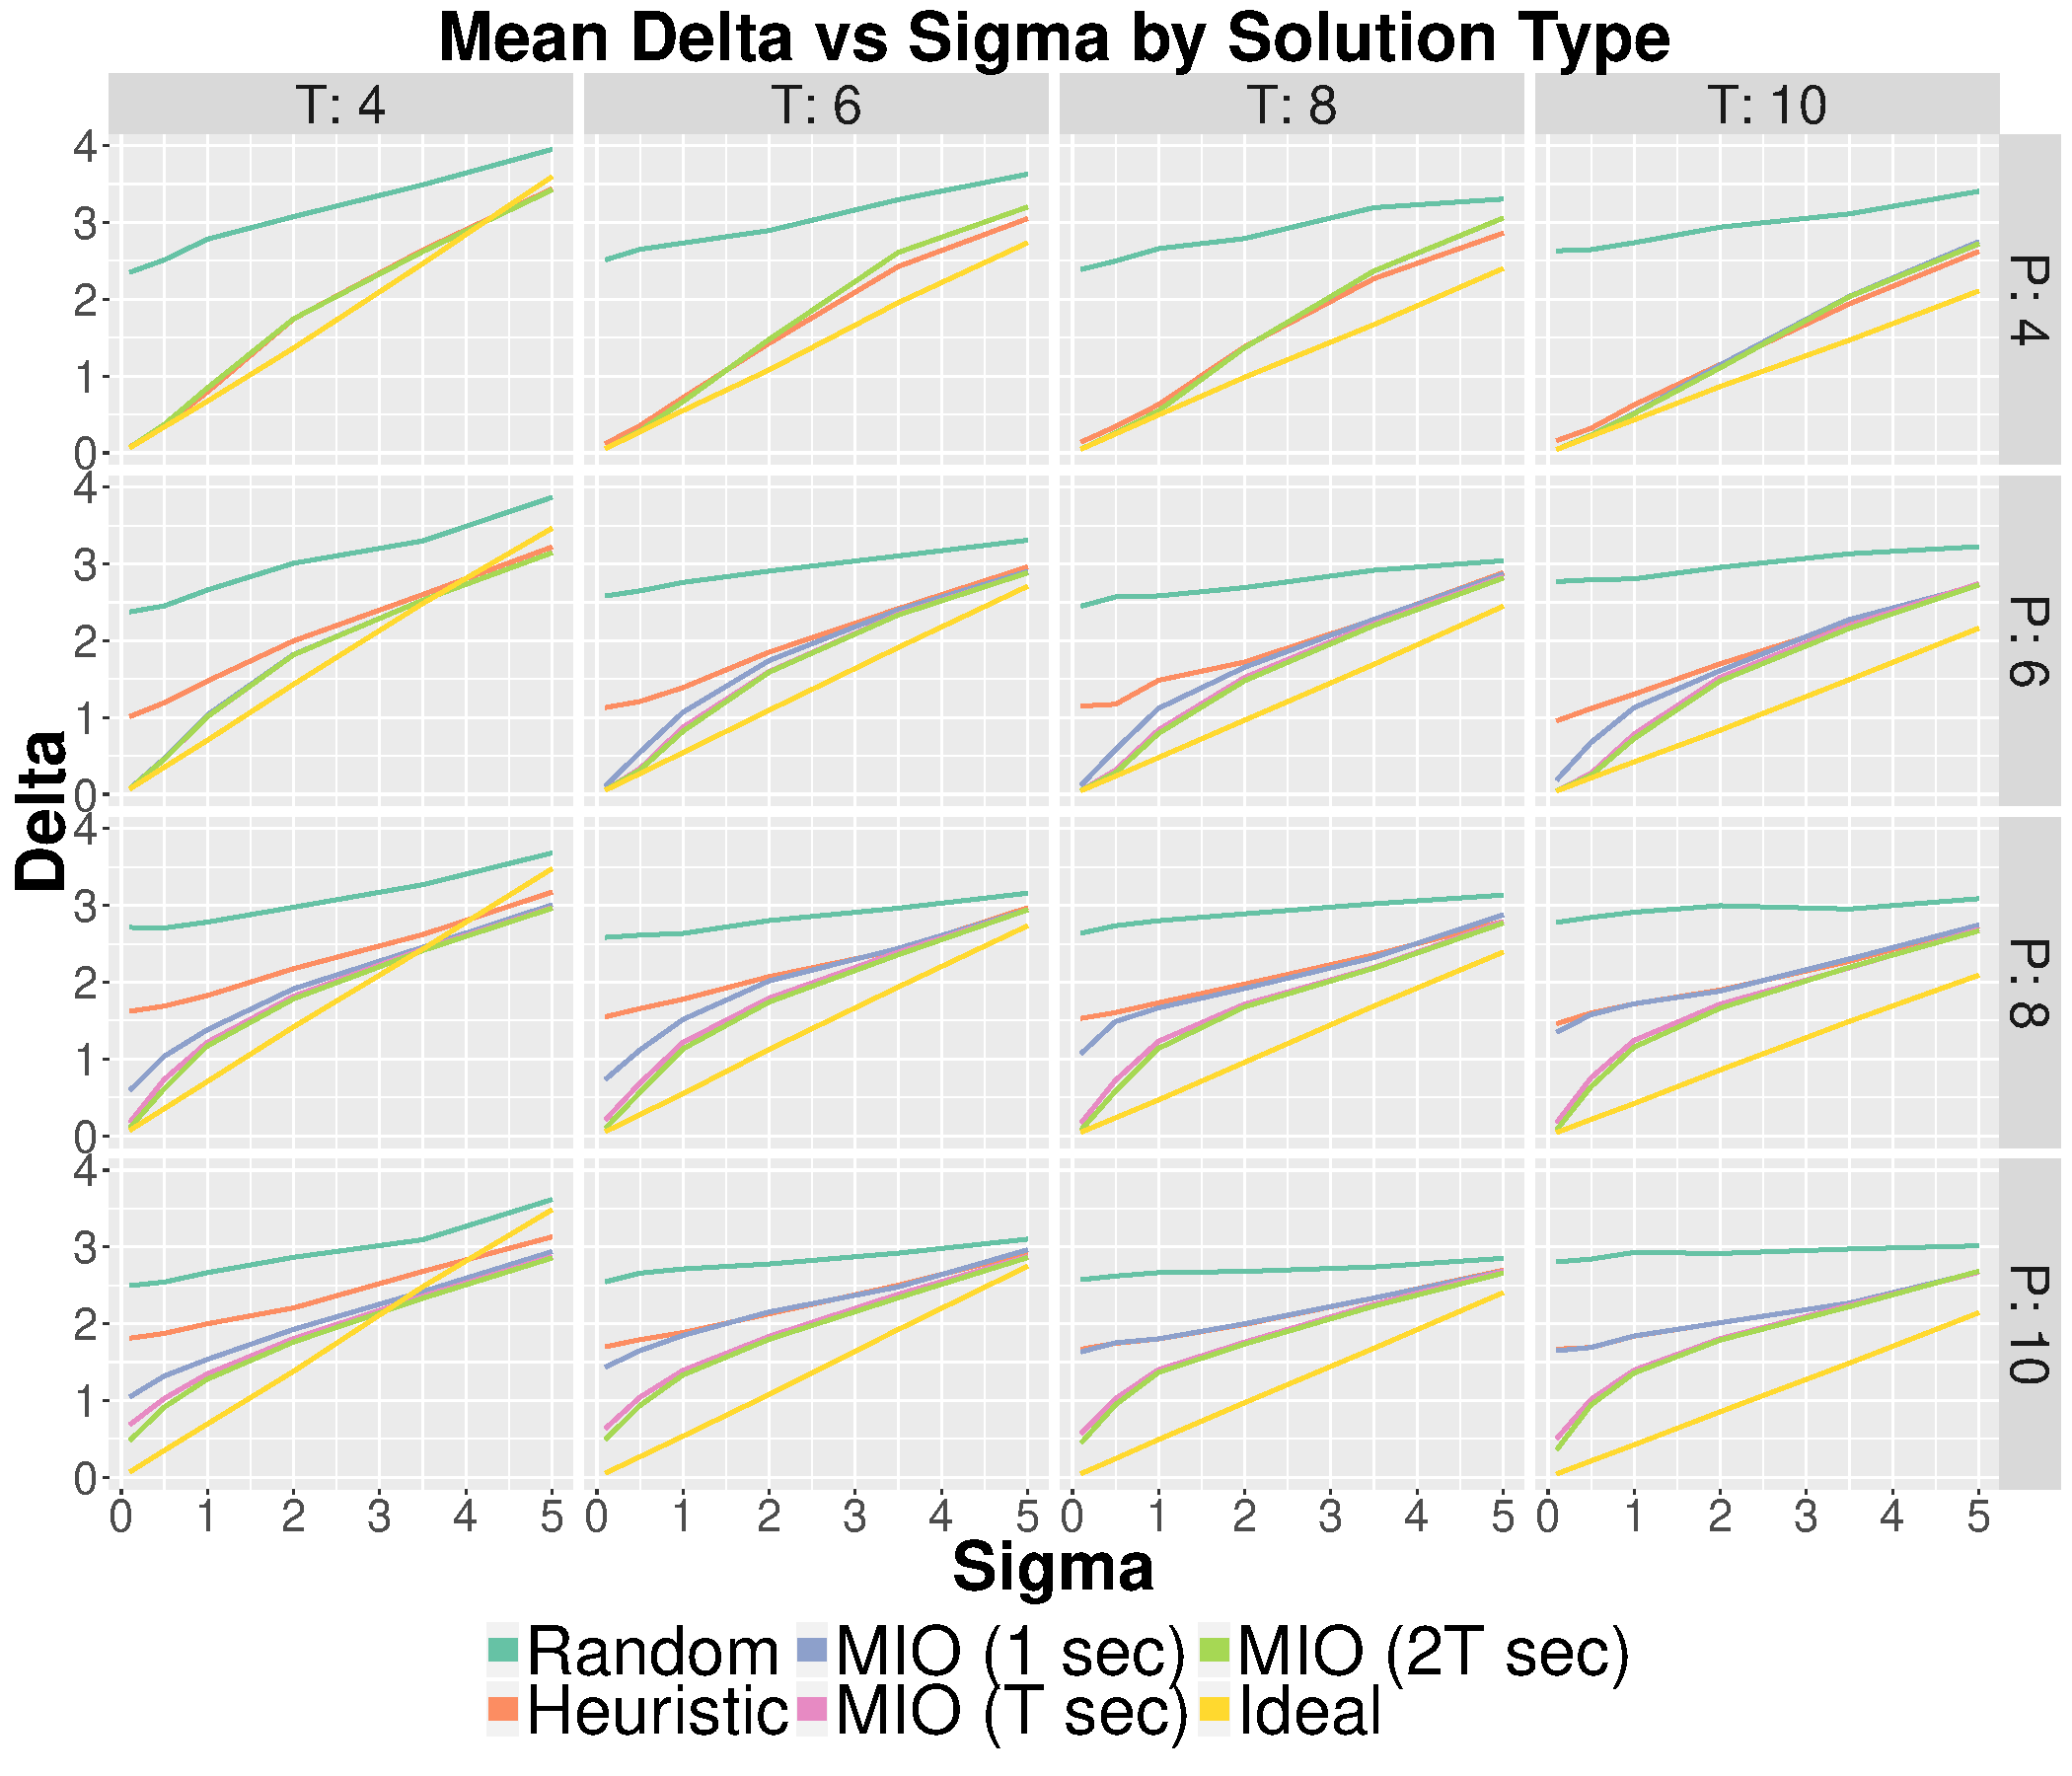
\includegraphics[width=\columnwidth]{../Figures/Basic_Delta_Summary}
  \caption{Trajectory estimation performance}
  \label{Fig:Basic_Delta_Summary}
\end{figure}

Remember that lower values of delta correspond to trajectory estimations that are closer to that of the true ground track. We note that as $\sigma$ approaches zero, both the heuristic and MIO trajectory estimates approach the trajectory estimates of the ideal solution, suggesting that both algorithms find very high quality trajectory estimates in these cases. Similar to the data association, it can be seen that the best estimates are reached after $1$ second for scenarios with four targets and after $T$ seconds for all other scenarios.

The heuristic and MIO outperform the ideal solution in scenarios with only four scans and high values of $\sigma$. However, the algorithms do not outperform the ideal solution for larger numbers of scans. Moreover, the ideal solution estimation changes linearly with sigma, but the slope of this linear dependence decreases as the number of scans increases. This suggests that as the number of scans approaches infinity, the estimated trajectories given by the ideal association will converge to the true ground tracks, even for large sigma values. This is also true for the MIO and heuristic solutions but to a lesser extent, which can be seen by the fact they move further away from the ideal solution when the number of scan increase, showing the tradeoff between added information and computational complexity.

We that the MIO and heuristic solutions estimation error have a bounded distance from the ideal one, and is always outperforms the random solution even for large values of $\sigma$. Which implies that though we do not necessarily get the optimal solution, the guiding objective prevents us from finding solution which are very poor. In particular, the gap between the ideal estimation error and the heuristic/MIO estimation error remains relatively constant across all values of $P$ for a fixed number of scans. 

\mysubsubsection{Summary of Results}
We have shown that in the case of no detection ambiguity
\begin{itemize}
\item The heuristic is highly scalable, and we can finds good quality solutions in fractions of a second using parallelization. 
\item Using these solutions as a warm start, the MIO achieves high quality solutions to both the data association and trajectory estimation measures after $T$ or fewer seconds. 
\item The MIO is scalable with respect to increases in both the number of targets and scans. We have also identified that there exists a tradeoff between making correct data associations and improved trajectory estimation, particularly in cases of high signal to noise ratios. 
\item Increasing the number of scans, while adding computational complexity to the model, helps to obtain better solutions. 
\end{itemize}
With these points in mind, we advance to discussing the case of scenarios with detection ambiguity. 

\mysubsection{Scenarios with Detection Ambiguity}
Here we extend our discussion to analyze the performance of our methods on scenarios with detection ambiguity. We first summarize our experimental methods before discussing performance of both the robust heuristic and the robust MIO in the spheres of both the data association and trajectory estimation problems.

This experiment serves as an extension of the basic one, in order to test the performance of our algorithms under detection ambiguity. We use the same scenarios generated from the basic experiment, however due to the additional difficulty inherent with detection ambiguity, we limit the range of signal noise to $\sigma \in \{0.1,0.5,1.0,2.0\}$, choosing to exclude the extreme cases of signal noise. In addition, we simulate both missed detections and false alarms. A detection is removed with probability, $\gamma$, and we consider $\gamma \in \{0.2,0.15,0.1,0.05\}$. We do not allow empty scans. For each scan, we generate false alarms according to a poisson distribution with parameter, $\lambda$, and false alarm locations are randomly selected uniformly within the state space. We consider $\lambda \in \{0.1,0.5,0.1,2.0\}$. The false alarms are then added to $\mathcal{X}_{t}$ and the detection order of $\mathcal{X}_{t}$ is randomly shuffled in the same manner as the first experiment. 

Once the data has been generated, we follow the same sequence of steps as outlined for the basic experiment, running the heuristic first and then feeding the solution into the MIO as a warm start. Note that the heuristic is only initialized with 1,000 starting points, as determined from the results of the basic experiment. Once again, the optimization process was set to terminate after $2T$ seconds, with solutions collected at intervals of $\{1,T,2T\}$ seconds. Prior to the running of this experiment, we performed a mini experiment and used the results to tune the penalties $\theta$ and $\phi$, a summary of the exact penalties used along with an explanation of the insight behind them, can be found in Appendix~\ref{app:Penalty_Appendix}. An important thing to note with regard to the penalties is that while the estimation error and the number of missed detections are highly correlated with the number of targets, the number of false alarms are not, and so the penalty $\theta$ is set to be linearly dependent on the number of estimated targets. In order to decide on the final estimated target number, we compared the average performance, i.e., the MIO objective function divided by the estimated number of targets, and chose the best one. 

\mysubsubsection{Robust Heuristic} Table~\ref{tab:Robust_heuristic_times} summarizes the minimum, mean, and maximum run times of the heuristic from the robust heuristic for a single starting point, arranged by the number of estimated targets ($P_{\text{est}}$) and number of scans ($T$). Times are shown in milliseconds. 
\begin{table}[ht]
\centering
\begin{tabular}{cc|ccc}
  \hline
   & & \multicolumn{3}{c}{Robust Heuristic Run Times} \\
   & & \multicolumn{3}{c}{(in milliseconds)}\\
   $ P_{\text{estimated}}$ & T & $\;\;$Min$\;\;$ & Mean & Max \\ 
  \hline
  \hline
  2 & 4 & 0.15 & 0.23 & 0.41 \\ 
  2 & 6 & 0.42 & 0.56 & 0.93 \\ 
  2 & 8 & 0.77 & 1.04 & 2.24 \\ 
  2 & 10 & 1.27 & 1.73 & 3.07 \\ 
  4 & 4 & 0.15 & 0.34 & 1.04 \\ 
  4 & 6 & 0.50 & 0.94 & 2.69 \\ 
  4 & 8 & 1.09 & 1.88 & 3.87 \\ 
  4 & 10 & 2.12 & 3.25 & 7.20 \\ 
  6 & 4 & 0.14 & 0.42 & 0.96 \\ 
  6 & 6 & 0.57 & 1.29 & 4.45 \\ 
  6 & 8 & 1.33 & 2.66 & 5.82 \\ 
  6 & 10 & 2.53 & 4.61 & 9.4 \\ 
  8 & 4 & 0.16 & 0.50 & 1.10 \\ 
  8 & 6 & 0.60 & 1.59 & 3.46 \\ 
  8 & 8 & 1.38 & 3.37 & 6.87 \\ 
  8 & 10 & 2.63 & 5.84 & 12.40 \\ 
  10 & 4 & 0.18 & 0.55 & 1.10 \\ 
  10 & 6 & 0.72 & 1.82 & 3.98 \\ 
  10 & 8 & 1.53 & 3.96 & 8.18 \\ 
  10 & 10 & 3.42 & 6.93 & 13.93 \\ 
  12 & 4 & 0.16 & 0.56 & 0.99 \\ 
  12 & 6 & 0.99 & 1.95 & 3.96 \\ 
  12 & 8 & 1.74 & 4.33 & 8.69 \\ 
  12 & 10 & 3.40 & 7.71 & 15.10 \\ 
   \hline
\end{tabular}
\caption{Robust heuristic run times (in milliseconds) for a single starting point.}
\label{tab:Robust_heuristic_times}
\end{table}

As expected, the robust heuristic requires longer run times than the basic heuristic, due to the increase in combinatorial solutions to the assignment problem. Comparing Table~\ref{tab:Basic_heuristic_times} and Table~\ref{tab:Robust_heuristic_times} we see that robust run times for four estimated targets are roughly four times longer than the corresponding run times in the basic heuristic for a fixed number of scans. However, the magnitude of this effect appears to decay as the number of targets increases. For example, in the case of eight targets, the robust heuristic times are only about twice that of the basic heuristic. This suggests that the robust heuristic still scales well with increases in the number of targets. It is also important to note that the run time variance in the robust case is much wider than the one for the basic case. However, parallelization might somewhat relieve this issue enabling the actual runtime to e closer to the average.

As exhibited by the basic heuristic, the scalability with regard to $P_{\text{est}}$ is better than with regard to $T$. For example, increasing from eight to ten scans for eight targets increases the computational cost by $140\%$, while increasing from eight to ten targets for eight scans increases the computational cost by $50\%$. Here, we must remind the reader, that for each scenario we actually have to check several $P_{\text{est}}$ values, which requires additional processing time and parallelization. In our simulations, we found that the range of possible $P_{\text{est}}$ values was generally limited to six values. 

\mysubsubsection{Number of Targets}
In the case of detection ambiguity, in order to correctly estimate the trajectories we must first correctly estimate the number of targets, consequently making this task extremely important. Therefore, we begin our analysis of detection ambiguity by evaluating the difference between the true and estimated number of targets. Explicitly, we define:
\begin{align}
	P_{\text{diff}} = P_{\text{true}} - P_{\text{est}},
\end{align}
where $P_{\text{est}}$ is the number of estimated targets and $ P_{\text{true}}$ is the number of true targets. Note that $P_{\text{diff}} = 0$ indicates that we have correctly estimated the number of targets. When $P_{\text{diff}} < 0$, we have overestimated the number of targets, whereas when $P_{\text{diff}} > 0$, we have underestimated the number of targets. Figure~\ref{fig:Robust_4_8_Histogram} plots the distribution of $P_{\text{diff}}$ for scenarios with four targets and eight scans, and for comparison, Figure~\ref{fig:Robust_8_8_Histogram} plots the same result for scenarios of eight targets and eight time scans. 
\begin{figure}[ht]
  \centering
  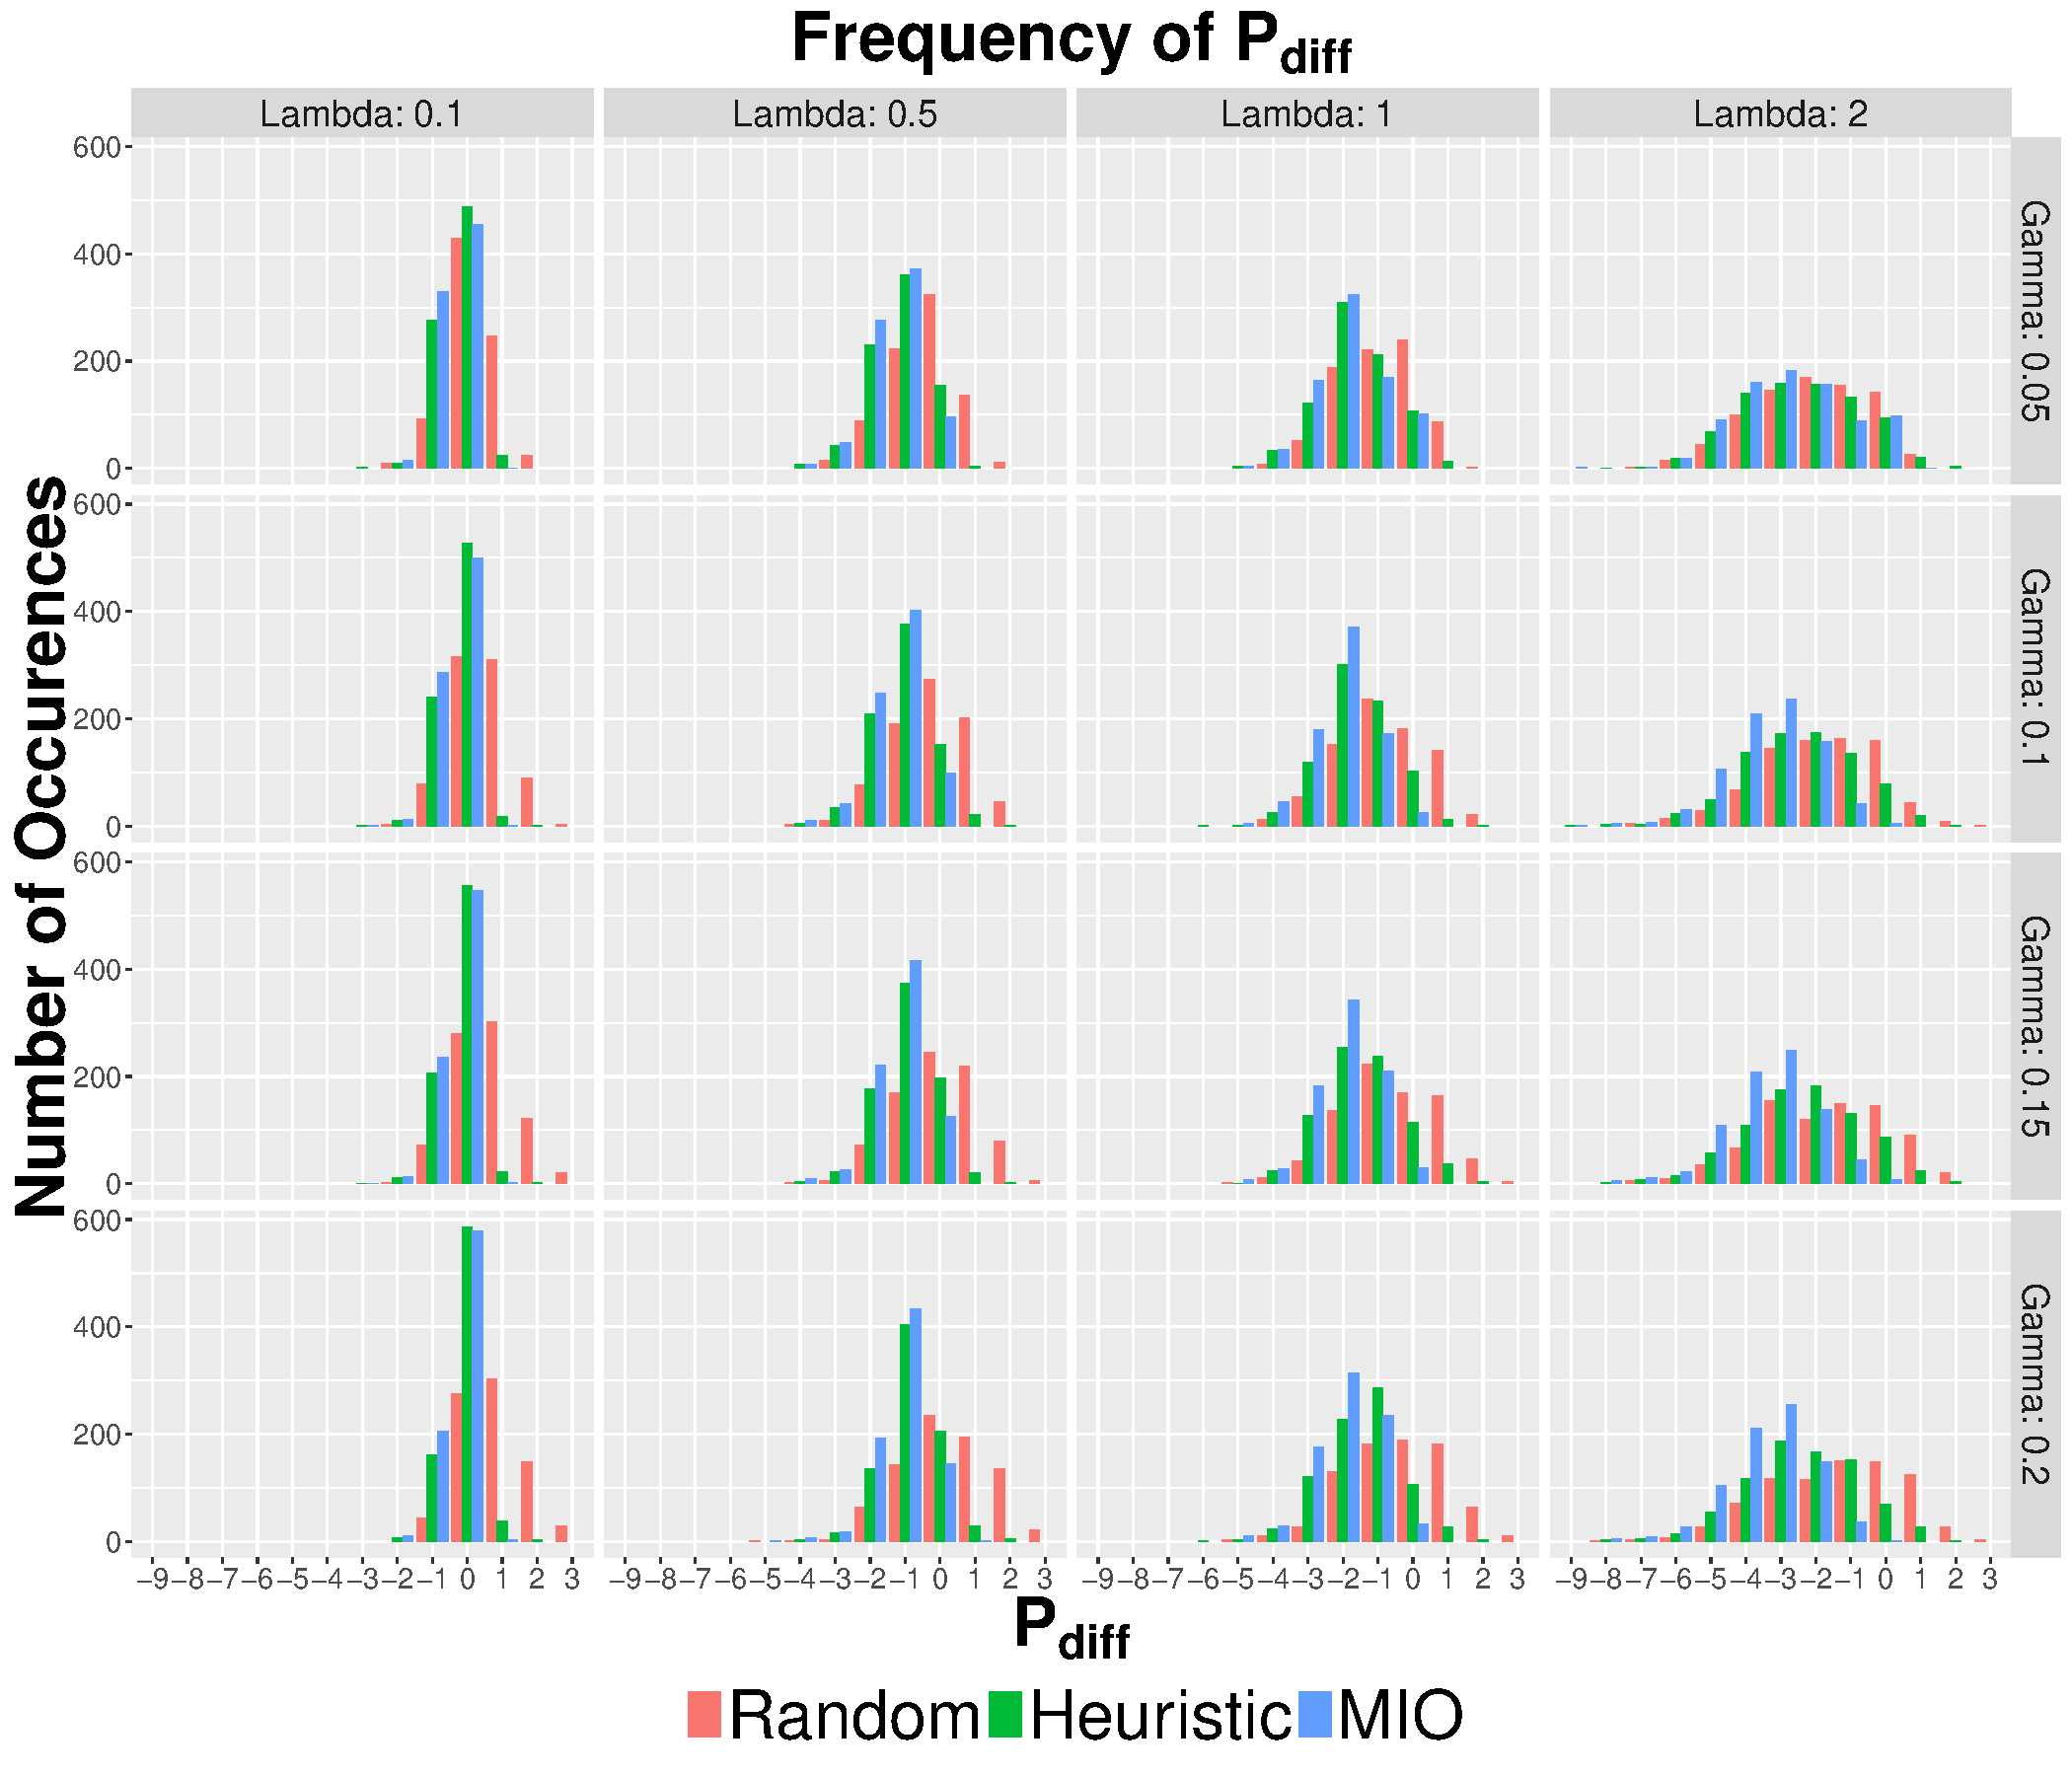
\includegraphics[width=\columnwidth]{../Figures/4_8_Histogram}
  \caption{Distribution of the difference in true and estimated number of targets for scenarios with 4 targets and 8 scans, arranged by $\gamma$ and $\lambda$.}
  \label{fig:Robust_4_8_Histogram}
\end{figure}
\begin{figure}[ht]
  \centering
  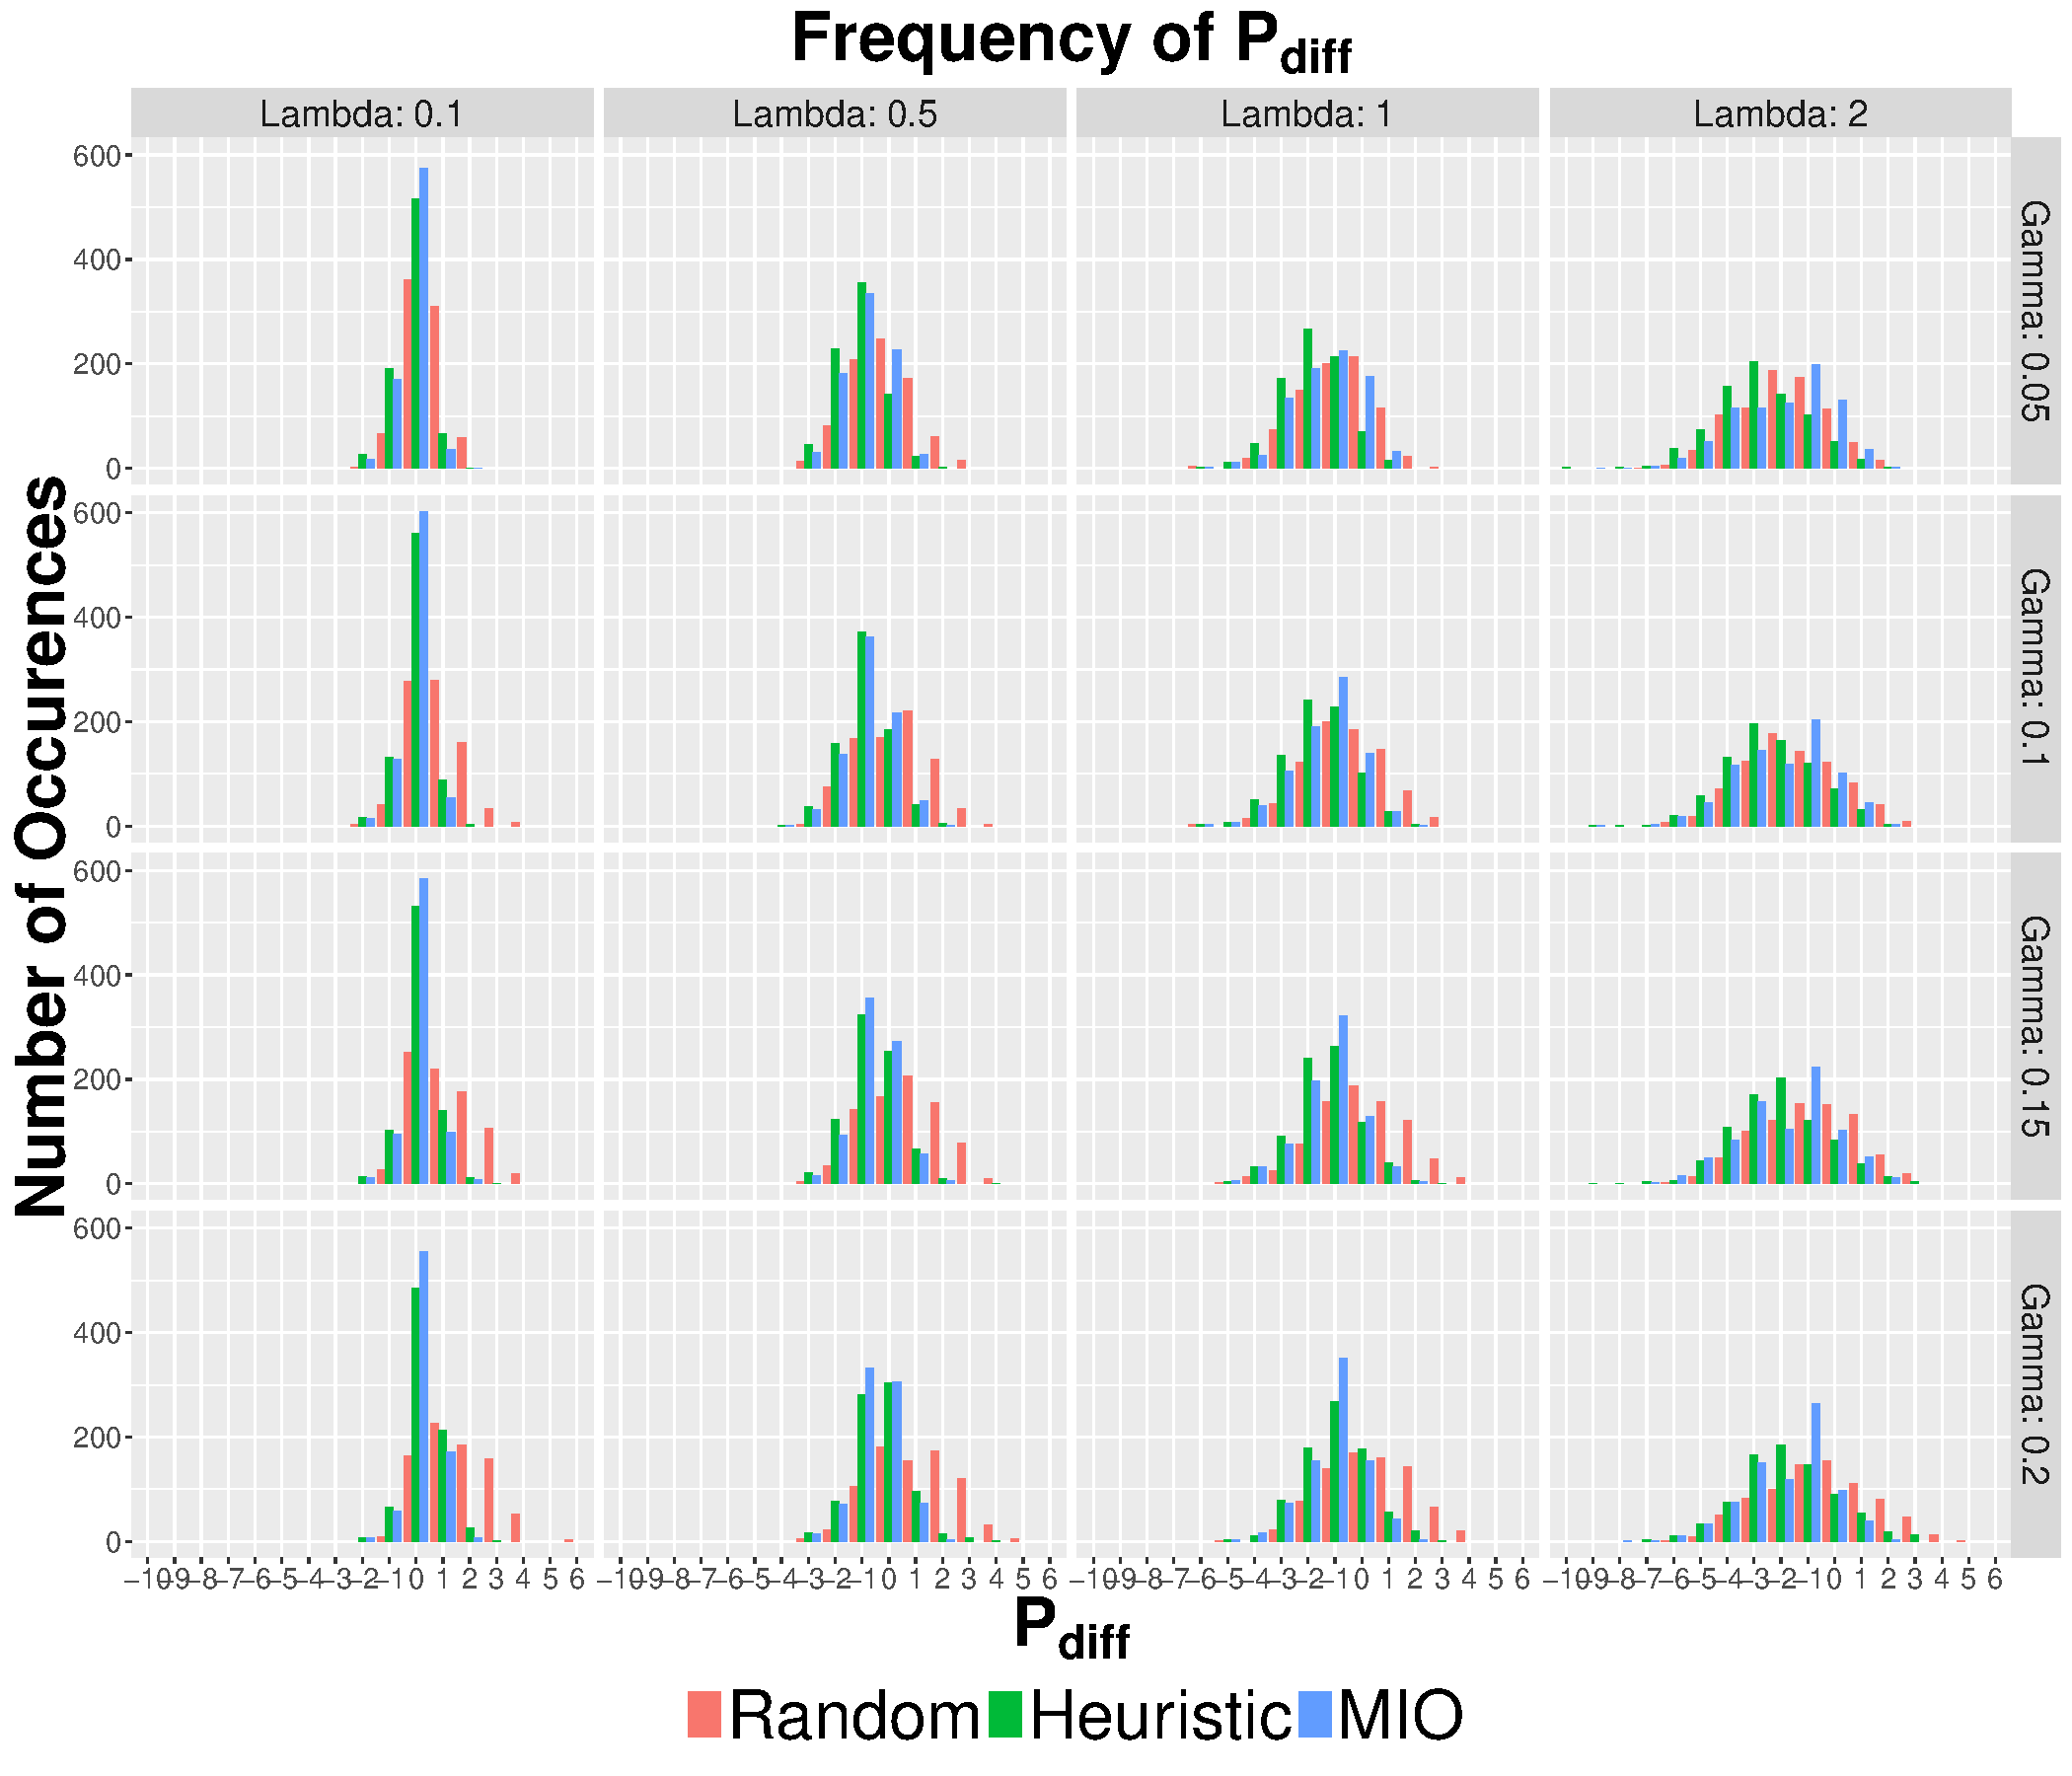
\includegraphics[width=\columnwidth]{../Figures/8_8_Histogram}
  \caption{Distribution of the difference in true and estimated number of targets for scenarios with 8 targets and 8 scans, arranged by $\gamma$ and $\lambda$.}
  \label{fig:Robust_8_8_Histogram}
\end{figure}

We see that both the robust heuristic and the robust MIO estimate the number of targets correctly a very high proportion of the time in both scenario sizes when $\lambda = 0.1$. As $\lambda$ increases, we see a tendency to overestimate the number of targets. This trend appears to be more prominent in Figure~\ref{fig:Robust_4_8_Histogram}, meaning that the scenario with four targets has a higher tendency to overestimate for large values of $\lambda$ than the scenario with eight targets. Further examination shows that both solutions have slightly fewer false alarms than the ideal solution for scenarios with eight targets, and this effect is slightly more exaggerated for the scenarios with four targets. This suggest that $\theta$ was set too high, or alternatively that, the missed detection penalty $\phi$ was too low, which is also supported by the fact that both algorithms identified too many missed detections. Altogether, this suggests that the algorithms likely took a preference to create additional trajectories misclassifying the false alarms as detections for these targets as well as assigning them many missed detections, ultimately resulting in a tendency to overestimate the number of targets. A finer tuning of $\theta$ and $\phi$ can resolve this problem, however, we find it difficult to tune these parameters for higher levels of the false alarm rate $\lambda$, which explains why this over estimation is worse as $\lambda$ increases. Moreover, it is difficult to tune the parameters to obtains the same tendencies for different number of targets, however, we do not know the true  number of targets, which leads us to believe that more sophisticated penalty functions are needed to neutralize this difference.

\mysubsubsection{Data Association}
Knowing that we tend to overestimate the number of targets with the given penalties, we move on in our analysis to measuring the accuracy of our robust approaches. Figures~\ref{fig:Robust_4_8_Accuracy} and~\ref{fig:Robust_8_8_Accuracy} plot accuracy against the difficulty metric, $\rho$, for scenarios of four and eight targets, respectively. Both scenarios have eight scans and both figures have been arranged by $\gamma$ and $\lambda$.
\begin{figure}[ht]
  \centering
  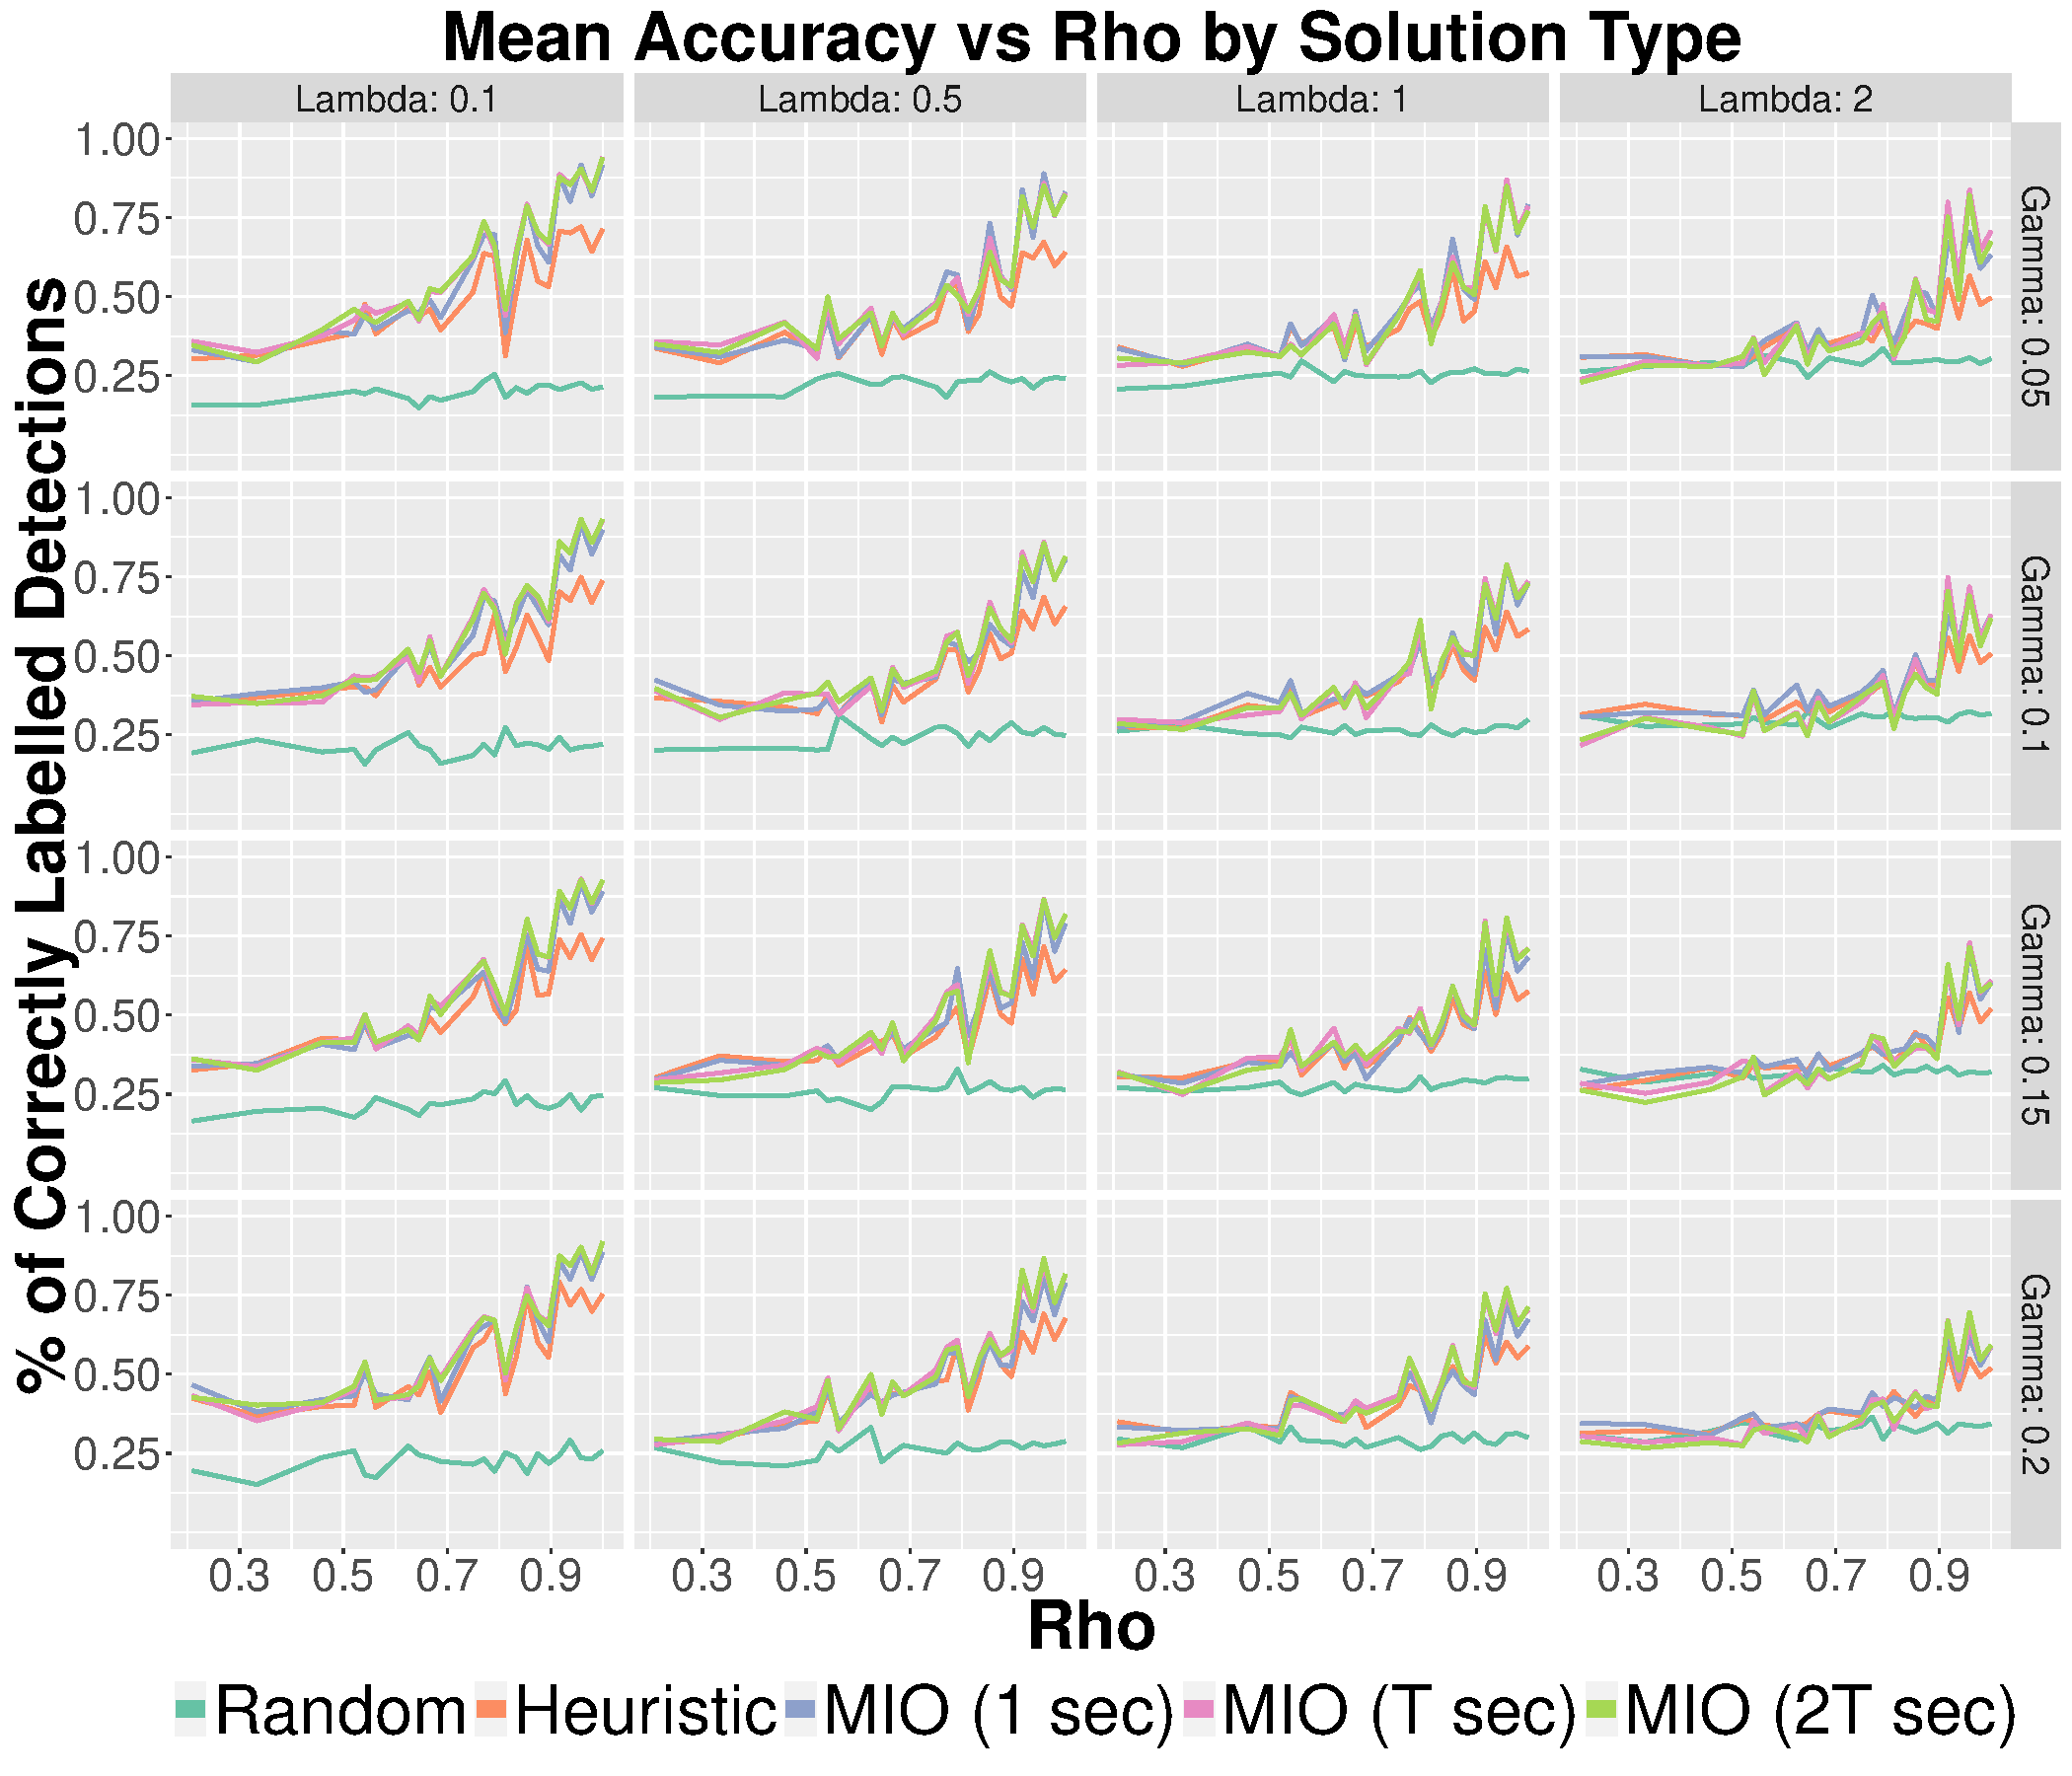
\includegraphics[width=\columnwidth]{../Figures/4_8_Accuracy}
  \caption{Accuracy of robust heuristic and MIO as compared to random solutions for scenarios of 4 targets and 8 scans, arranged by $\gamma$ and $\lambda$.}
  \label{fig:Robust_4_8_Accuracy}
\end{figure}
\begin{figure}[ht]
  \centering
  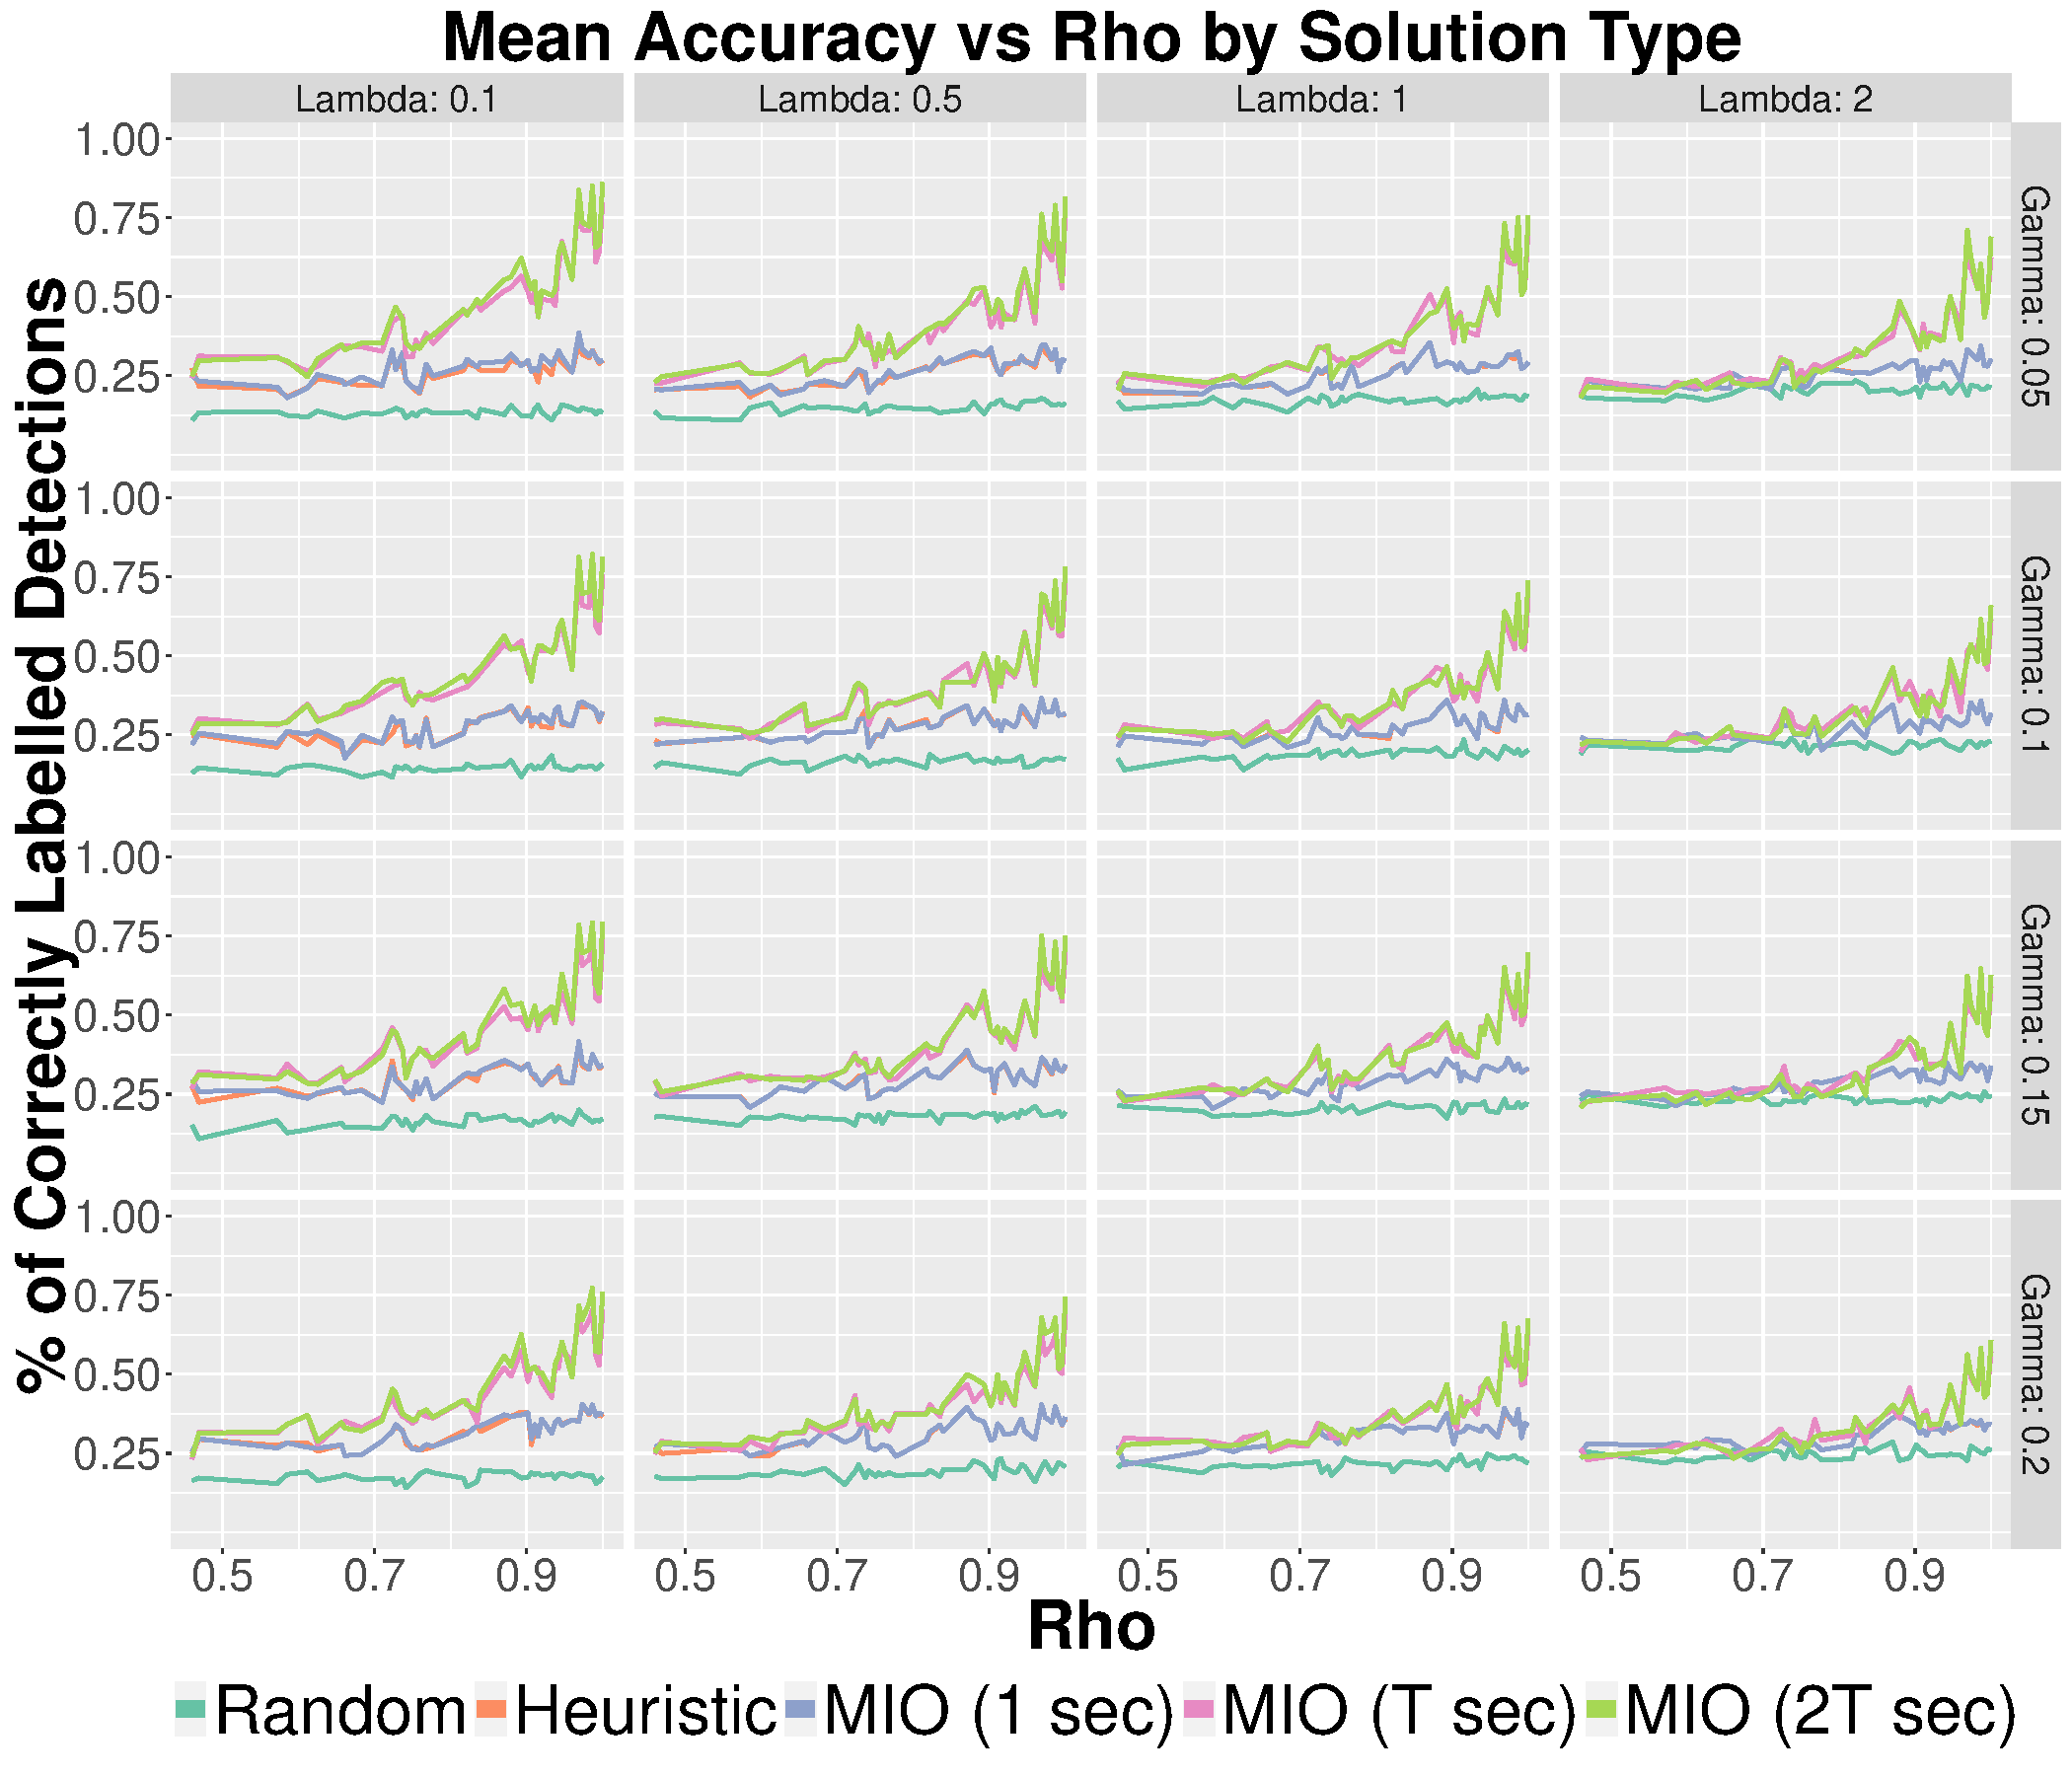
\includegraphics[width=\columnwidth]{../Figures/8_8_Accuracy}
  \caption{Accuracy of robust heuristic and MIO as compared to random solutions for scenarios of 8 targets and 8 scans, arranged by $\gamma$ and $\lambda$.}
  \label{fig:Robust_8_8_Accuracy}
\end{figure}

In Figure~\ref{fig:Robust_4_8_Accuracy} we see the accuracy results for four targets. In this case the heuristic solution is an significant improvement over the random solution, and is close to the best solution achieved by the MIO. The MIO achieves this best solution after 1 seconds, and no significant improvement is offered by running it for a longer period. In comparison, the accuracy in the eight targets scenarios, which is seen in Figure~\ref{fig:Robust_8_8_Accuracy}, the heuristic offers a smaller improvement to the random solution, and the MIO improves upon the heuristic solution only  after $T$ seconds, reaching its best accuracy. 

As we stated earlier, even with small values of $\lambda$ and $\gamma$ the case of detection ambiguity has an added difficulty of estimating the correct number of targets. Therefore, the fact that for $\lambda=0.1$ and $\gamma=0.05$ the decrease of accuracy with regard to the basic solution decreases by $5\%-10\%$ for both four and eight targets and across scenario difficulties suggests that we deal  well with this issue. Moreover, in the case of four target we reach a accuracy level above $90\%$  even for the highest value of $\gamma$ (where it was almost $100\%$ for the basic scenarios), suggesting that we are very close to the ideal association.

The robust approaches also appear to be more sensitive to higher false detection rates than higher missed detection probabilities. For example, for eight targets, fixing $\gamma=.05$, the MIO after $T$ accuracy decreases from about $90\%$ to $65\%$ when increasing $\lambda$ from $0.1$ to $2.0$, while fixing $\lambda=.1$ and increasing $\gamma$ from $.05$ to $.2$ reduces accuracy to $75\%$. This can also be attributed to our difficulty in tuning the penalties for higher levels of $\lambda$, which in turn, caused an over estimation of the number of targets, and therefore a reduced accuracy. 

\mysubsubsection{Trajectory Estimation}
We conclude our analysis of the robust approaches with a discussion on their performance in the sphere of the trajectory estimation problem. Figures~\ref{fig:Robust_4_8_Delta} and~\ref{fig:Robust_8_8_Delta} plot the $\delta$ performance metric against the detection error $\sigma$, for scenarios of four and eight targets, respectively. 
\begin{figure}[ht]
  \centering
  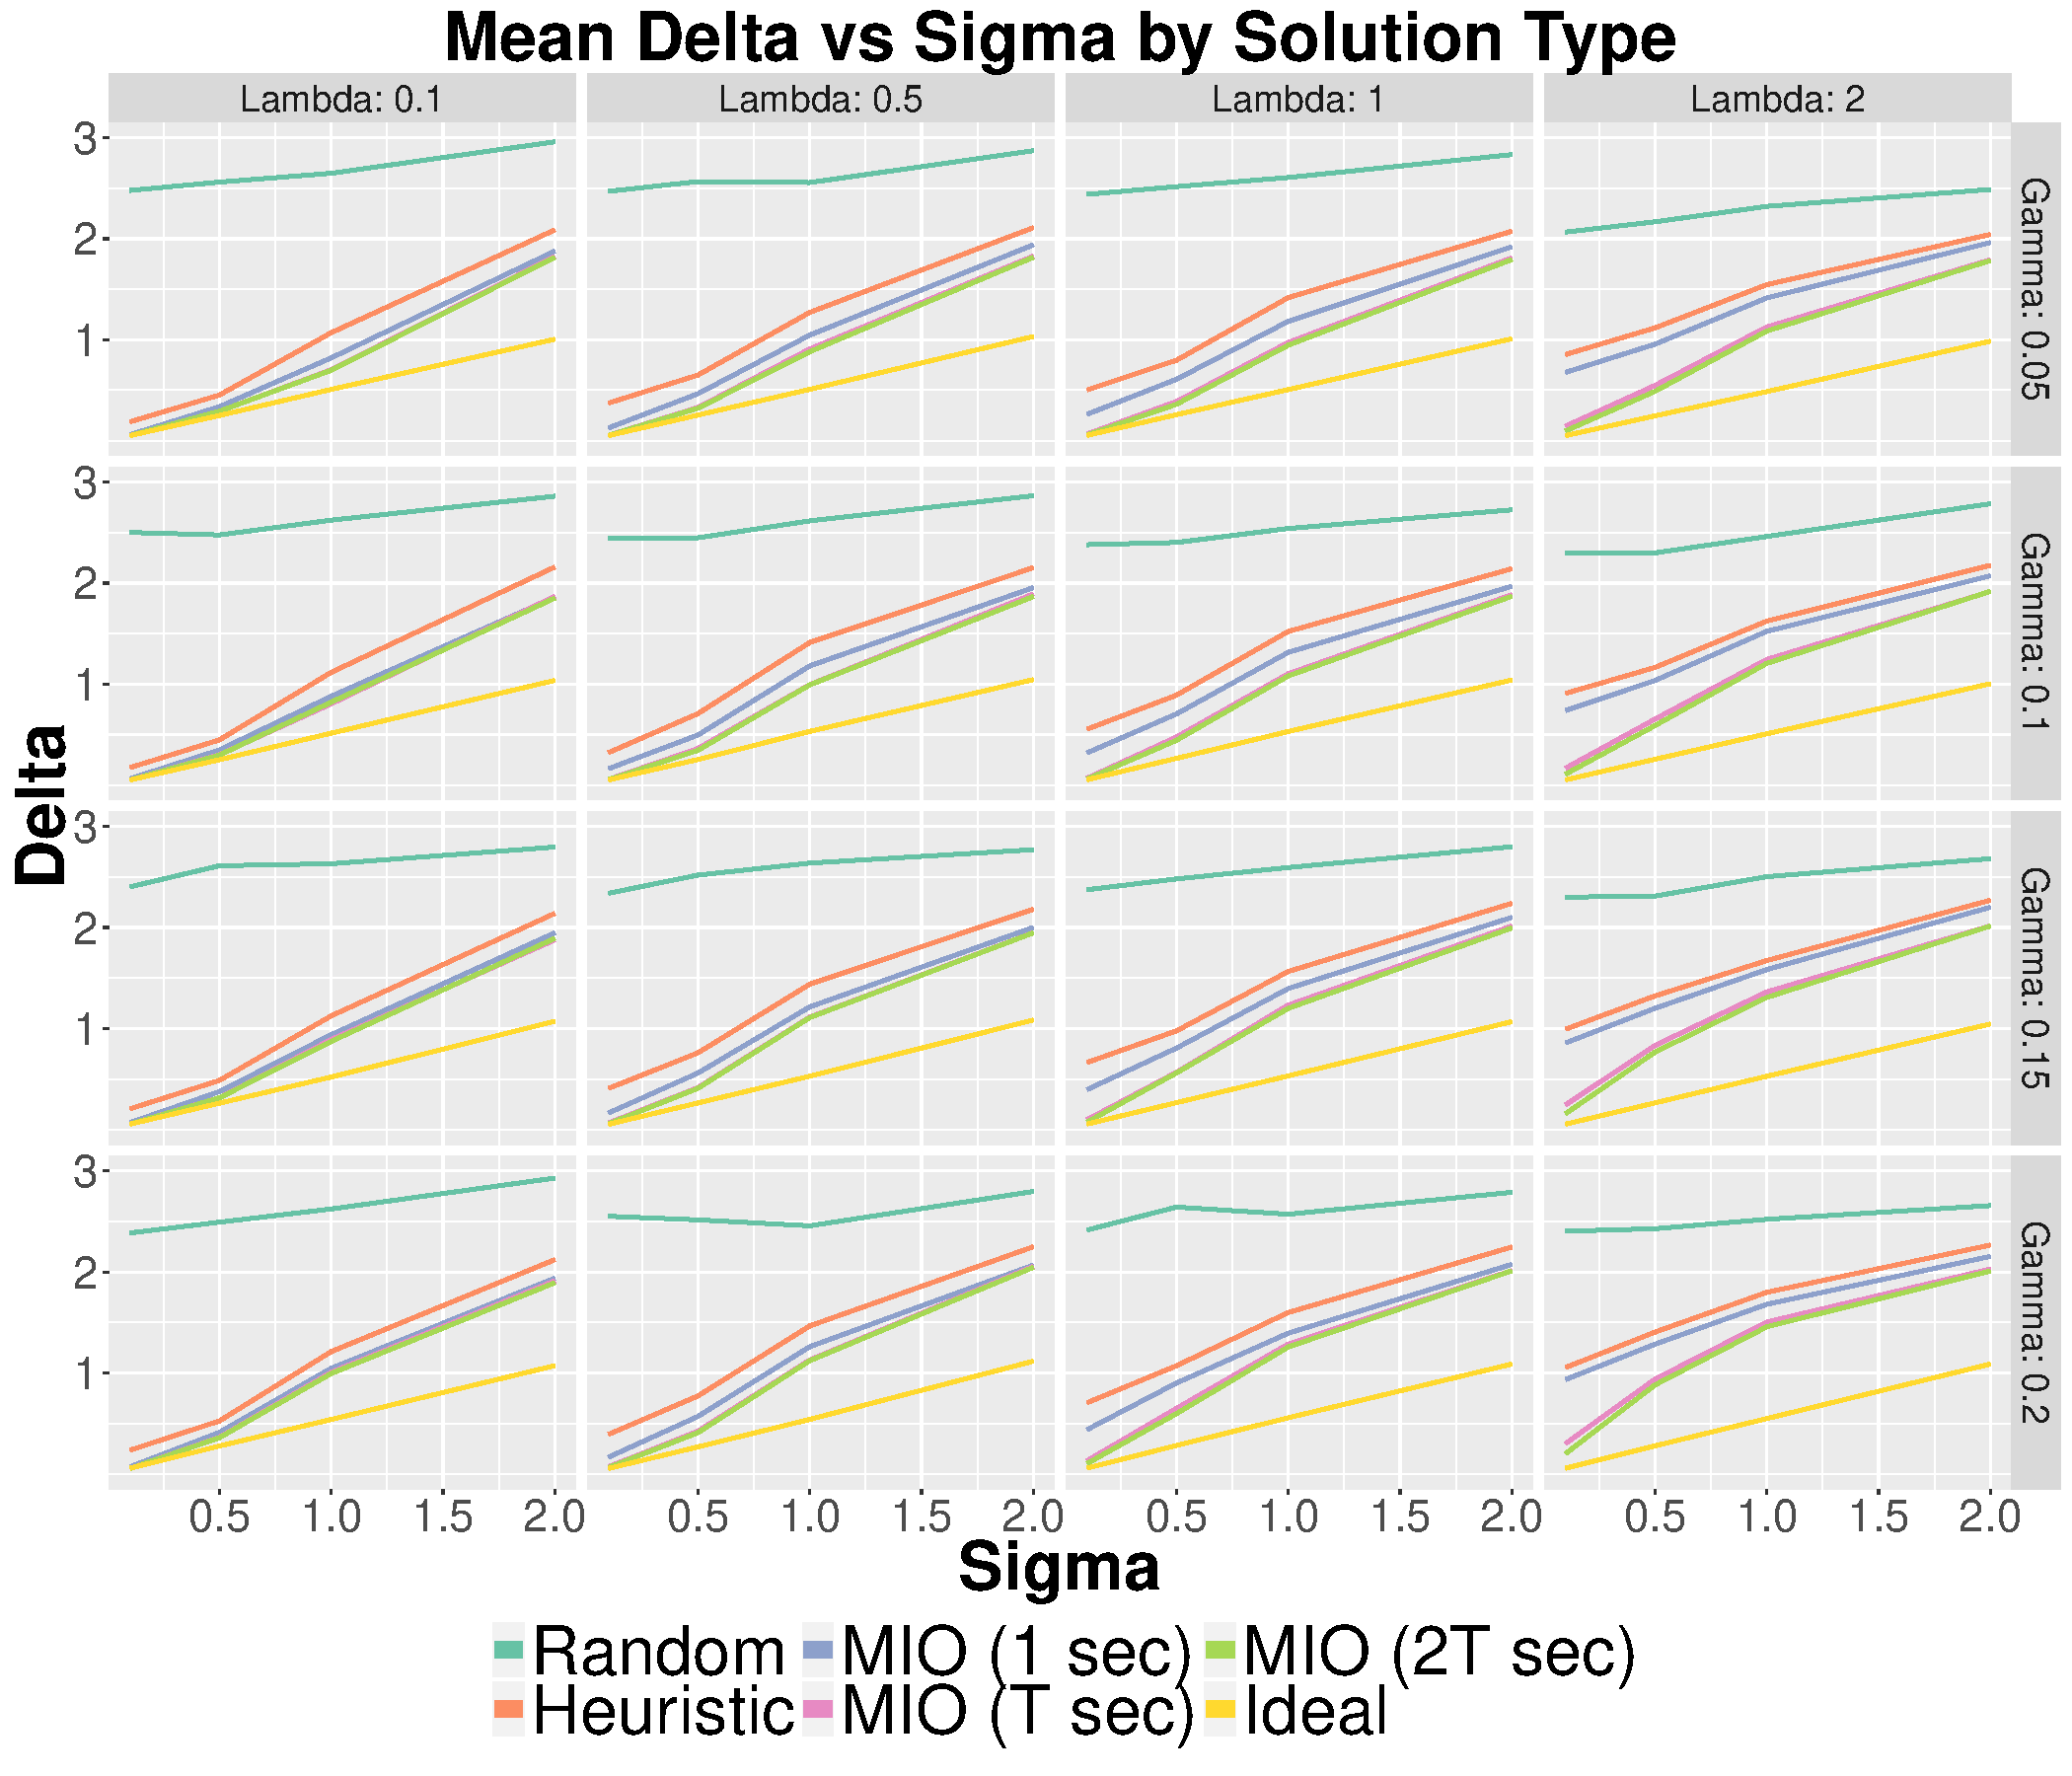
\includegraphics[width=\columnwidth]{../Figures/4_8_Delta}
  \caption{$\delta$ of robust heuristic and MIO as compared to random solutions for scenarios of 4 targets and 8 scans.}
  \label{fig:Robust_4_8_Delta}
\end{figure}
\begin{figure}[ht]
  \centering
  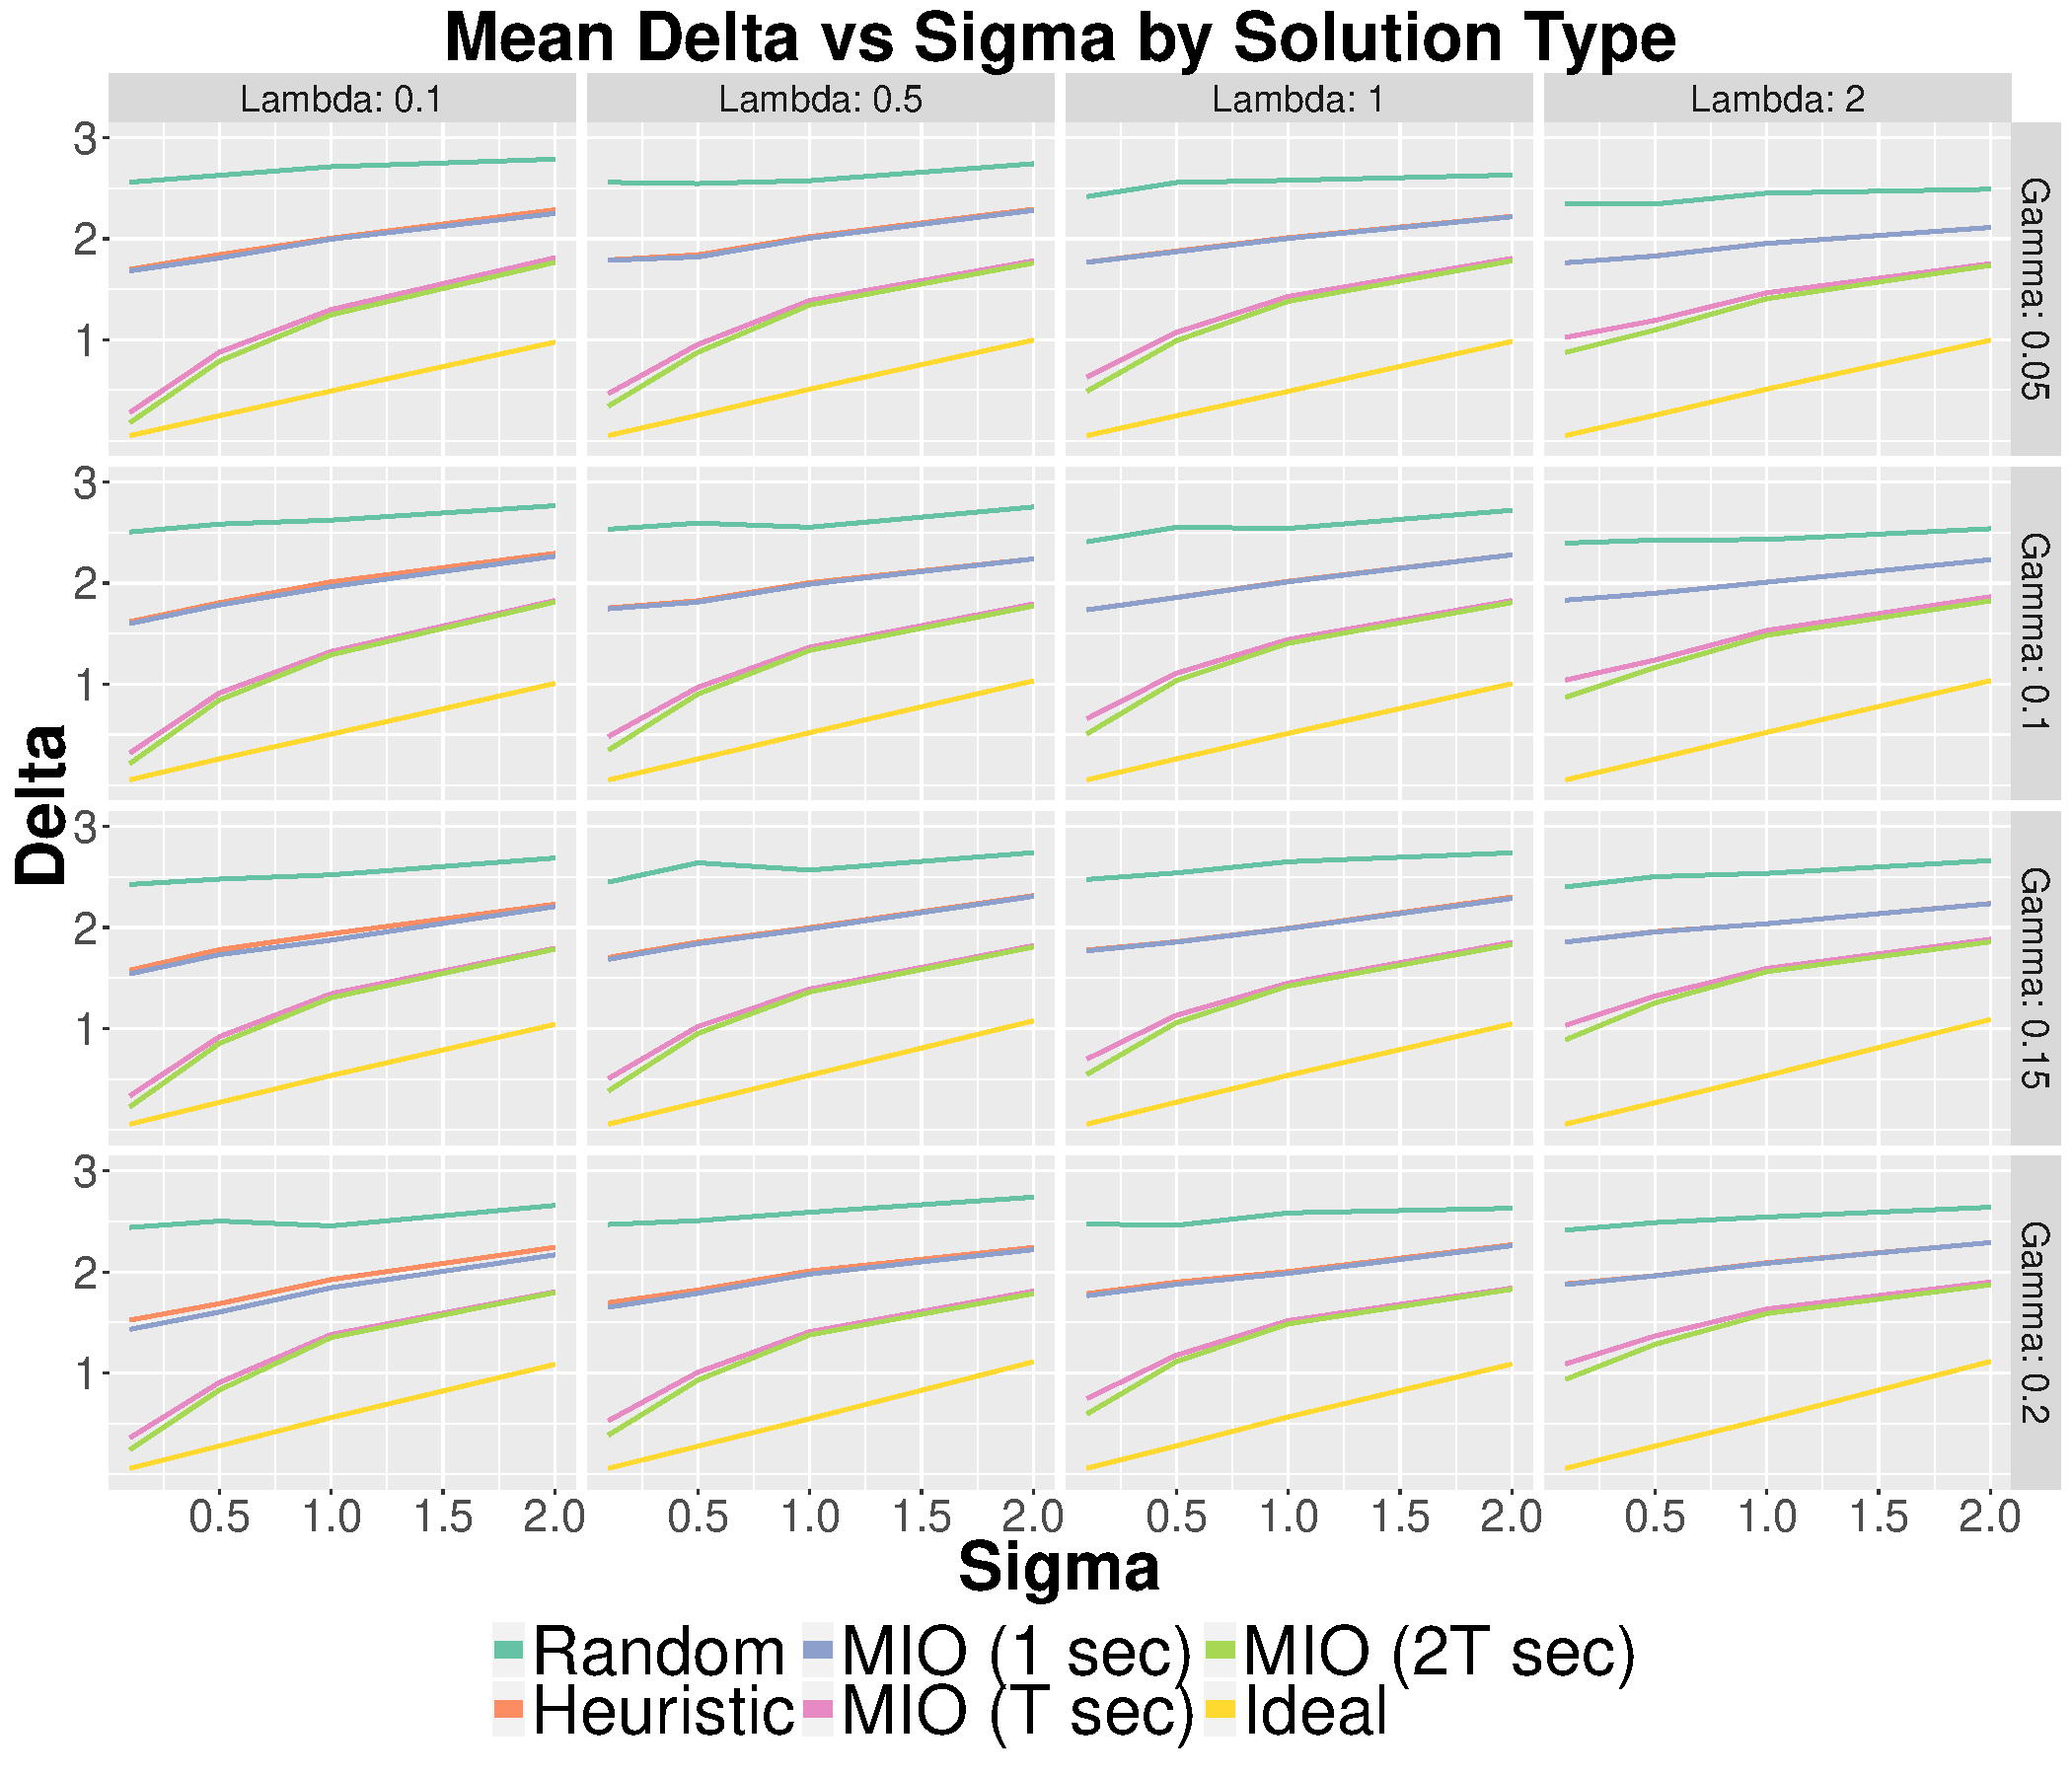
\includegraphics[width=\columnwidth]{../Figures/8_8_Delta}
  \caption{$\delta$ of robust heuristic and MIO as compared to random solutions for scenarios of 8 targets and 8 scans.}
  \label{fig:Robust_8_8_Delta}
\end{figure}

Note that $\delta$ is calculated using the $\min\{P_{\text{true}},P_{\text{est}}\}$. The fact that we tend to overestimate means that more often than not $\delta$ will be calculated using $P_{\text{true}}$. This implies that in most cases we match all the true trajectories to estimated ones, and so the number of trajectories for the $\delta$ calculation is the same as in the scenarios without detection ambiguity. Thus, we can compare and interpret their values directly.

In comparing Figure~\ref{fig:Robust_8_8_Delta} with the graph in Figure~\ref{Fig:Basic_Delta_Summary} corresponding to $P=8$ and $T=8$, we see that for $\lambda=0.1$ and $\gamma=0.05$ there is no observable loss of performance in adding the detection ambiguity, for the MIO after $T$ seconds. This observation also holds true for the heuristic solution. In contrast, comparing Figure~\ref{fig:Robust_4_8_Delta} with the graph in Figure~\ref{Fig:Basic_Delta_Summary} corresponding to $P=4$ and $T=8$, and the same $\lambda$ and $\gamma$ values, the $\delta$ value for the MIO increases for $\sigma$ values larger than $0.5$, and the increase becomes worse as $\sigma$ increases. Moreover, in the same case, the heuritic performance deteriorates even more sharply than the MIO's performance. 

Similar to what we have seen for the data association problem, in the trajectory estimation problem our approaches are also more robust to increases in $\gamma$ than increases in $\lambda$. Figures~\ref{fig:Robust_4_8_Delta} and~\ref{fig:Robust_8_8_Delta} both show that there is little to no loss in the quality of the trajectory estimation when increasing $\gamma$ for both the heuristic or MIO, and this holds true across all values of $\sigma$ and $\lambda$. Whereas, especially for small $\sigma$ values, as $\lambda$ increases we see the estimation of the MIO ran for $T$ seconds deteriorating, for example, for eight targets and $\sigma=0.1$, while for $\lambda=0.1$ we get $\delta$ close to zero, for $\lambda=2$ the value of delta increases to $1$.  This deterioration is a lot milder for the case of four targets.

\mysubsubsection{Detection Ambiguity Summary}
The case of detection ambiguity provides two additional challenges: the assignment problem is more complex for a fixed number of targets, and an added problem of deciding the correct number of target.
The results for this case indicate thats
\begin{itemize}
\item  Tuning the parameters leads to a correct estimation of the number of targets, even for a relatively large scenario.
\item The accuracy deteriorates by 5\%-10\% with the addition of detection ambiguity.
\item Although we tend to overestimate the number of targets, the quality of estimated trajectories that correspond to the true trajectories is similar to the case with no detection ambiguity.
\item The solution of the MIO is more robust to changes in missed detection probability than to changes in the false alarm rate.
\end{itemize}